\documentclass[pdftex,11pt,a4paper]{book}

\usepackage[spanish]{babel}
\usepackage[utf8]{inputenc}
\usepackage[pdftex]{graphicx}
\usepackage{url}
\usepackage[top=1.5in, bottom=1in, left=1in, right=1in]{geometry}
\usepackage{hyperref}
\usepackage{cite}
\usepackage{float}
\usepackage{eurosym} % para el euro
\usepackage{enumerate}

\newcommand{\HRule}{\rule{\linewidth}{0.5mm}}

\renewcommand\figurename{Imagen}


\begin{document}

\begin{titlepage}
\begin{center}

% Upper part of the page. The '~' is needed because \\
% only works if a paragraph has started.
% -----
%
\includegraphics[width=0.35\textwidth]{img/marca-uji-2955.png}~\\[2cm]

\includegraphics{img/marca-uji-2956.png}~\\[3.0cm]

\textsc{\LARGE Grado en Ingeniería Informática}\\[1.5cm]

\textsc{\LARGE Diseño e Implementación de Sistemas de Información}\\[1.5cm]
%%%%%%\textsc{\LARGE Versión Provisional}\\[1.5cm]

% Title
\HRule \\[0.4cm]
{ \huge \bfseries Sistema de soporte a la gestión de la Asignación de Proyectos en Empresas \\[0.4cm] }

\HRule \\[1.5cm]

% Author and supervisor
\begin{minipage}{0.4\textwidth}
\begin{flushleft} \large
\emph{Autor:}\\
Víctor \textsc{Sánchez Terrasa}
\end{flushleft}
\end{minipage}
\begin{minipage}{0.4\textwidth}
\begin{flushright} \large
\emph{Tutor académico:} \\
María de los Ángeles \textsc{López Malo}
\end{flushright}
\end{minipage}

\vfill

% Bottom of the page
% -----
% Sustituir los signos "\_" por lo que corresponda. 
{\large Fecha de lectura: 16 de julio de 2018\\
Curso académico 2017/2018}

\end{center}
\end{titlepage}
\setlength{\parskip}{\baselineskip}



% ------------------- Página resumen ---------------------

\thispagestyle{empty} % página sin numerar

\clearpage % Resumen y Palabras clave en página 2.

\section*{Resumen}

En el presente documento se recoge el trabajo realizado en la empresa EFI-Cretaprint tratándose sobre el desarrollo de una aplicación capaz de simular las funciones de un controlador lógico programable. Este controlador se encuentra en el interior de cada impresora de cartón corrugado encargado de controlar e informar del estado de las partes mecánicas. Las impresoras de cartón corrugado son fabricadas y vendidas por EFI-Cretaprint.

Las etapas del desarrollo de la aplicación que efectúa la función de controlador lógico programable dentro de la impresora, desde aquí en adelante PLC, se encuentran disponibles para el lector en el presente documento, con cada etapa como la definición del proyecto: documentación de los elementos necesitados para el desarrollo, requisitos del proyecto, análisis del proyecto, diseño de la aplicación, desarrollo, problemas que han surgido durante el desarrollo y puesta en marcha junto con la aplicación con la que ha de funcionar, así como también se encontrará al final una opinión del proyecto.

El alcance de este sistema incluye todo el manejo con el apartado del controlador lógico programable, pero no incluye los servicios de las capas de más nivel que interactúan con el usuario, al tratarse de una herramienta de uso interno para el desarrollo de la máquina.

La herramienta interna del departamento de desarrollo de software de la empresa es el principal motivo de todo el trabajo realizado. La necesidad de esta herramienta viene por el hecho que la empresa solo dispone de una impresora de desarrollo en la que se realizan las distintas pruebas de la siguiente generación de impresoras. Esta única impresora es utilizada por los distintos departamentos para la realización de pruebas, teniéndose que repartir las horas de pruebas entre los distintos empleados de cada departamento. A partir de este problema surge la idea de crear una aplicación capaz de simular la comunicación realizada con el PLC que dispone la impresora.

\section*{Palabras clave}

Simulador, modbus, PLC

\section*{Keywords}

Simulator, modbus, PLC

\thispagestyle{empty} % página sin numerar

\cleardoublepage


% ------------------- Página índice ---------------------


\pagestyle{plain} % todas las páginas numeradas, sin cabeceras. Sustituir por \pagestyle{headings} para añadir cabeceras a las páginas. 

\tableofcontents

\cleardoublepage

% ------------------- Cuerpo de la memoria ---------------------

\chapter{Introducción}

\section{Contexto del proyecto}

El proyecto cuya propuesta se presenta en este documento, se ha desarrollado en EFI-Cretaprint S.L.U. subsidiaria de la empresa multinacional Electronics for Imaging, Inc. (EFI) con una sede central de más de 3100 trabajadores ubicada en la ciudad de Fremont del estado de California, Estados Unidos. Dicha empresa dispone de principales subsidiarias importantes para el desarrollo de la compañía empleando un sistema de desarrollo Spring, proponiendo objetivos a corto plazo, así de esta forma corregir rápidamente los errores que se puedan encontrar durante su desarrollo. Con este sistema, EFI es la compañía líder mundial en el sector en la fabricación de impresoras de cartón corrugado gracias a la subsidiaria EFI-Cretaprint S.L.U. que tiene la sede principal en el Carrer dels Ibers nº 54 ubicado en el Polígono Industrial SUPOI 8 del municipio de Almazora, provincia de Castellón, para todo el territorio español. Con una cantidad en aumento de 80 trabajadores investigan, desarrollan y fabrican las impresoras de cartón corrugado de la compañía que se encuentran actualmente por todo el mundo.

EFI permite que EFI-Cretaprint S.L.U. pueda actuar con total autonomía en numerosos aspectos, como si se tratara de una empresa externa, empleando apoyo de la matriz EFI en ciertos tipos de recursos como pueden ser el uso de aplicaciones administrativas, correo electrónico, organigrama empresarial...  En el caso del organigrama empresarial, la empresa dispone de los departamentos básicos que requiere cualquier empresa en expansión: recursos humanos, contabilidad, inventario y administración. Después nos encontramos con los departamentos que le dan valor a la empresa en el mundo de investigación: software, ingeniería, estructuras, electricidad, mecánica, materiales y tintas. Todos estos departamentos trabajan de forma horizontal colaborando entre ellos cuando se cruzan las partes del proyecto. Cada departamento se divide en equipos especializados en una parte del desarrollo, para una mayor eficacia en la distribución de conocimientos, así como también tiene apoyo de empresas externas en las que los trabajadores de estas empresas externas cuentan como un trabajador más de EFI.

Las impresoras de EFI son capaces de imprimir tanto en cartón corrugado de diversas ondas como en cartón compacto. Dicho cartón es el que muchas veces envuelve aquellos productos que compramos en las tiendas de electrodomésticos, de ahí la demanda de este tipo de impresoras que con un tamaño de 180m\textsuperscript{2} poseen una tasa de impresión de hasta 75m/minuto lineales (unos 7224m\textsuperscript{2}/hora) con las que pintan las cajas contenedoras de los productos que tanto anhelamos tener en perfecto estado.

EFI investiga la creación de nuevas impresoras de cartón corrugado, siendo un producto que no se puede disponer en cuantía in situ por su gran tamaño y alto coste por cada unidad. Esto supone un problema a la hora de poder experimentar con ellas, generando muchos problemas para la continuación del proyecto. Por tanto una de las soluciones planteadas es la de simular la mayor cantidad de partes de la máquina, para que esta forma la dependencia física sea la menor posible.

\section{Motivación del proyecto}

Partiendo de la necesidad de depender lo mínimo posible de la impresora física en el momento de su desarrollo, al departamento de software de EFI se le ocurrió que sería una buena idea poder simular aquellos elementos que dependen de partes mecánicas de la impresora. Una de estas partes es el controlador lógico programable, también conocido en la industria como \emph{PLC}, que es el encargado de controlar los elementos mecánicos de la impresora.

El sistema debe permitir interactuar de la misma forma que con una impresora real, incluyendo los estados de funcionamiento en los que pudiera estar, generando los posibles errores y alarmas que puedan existir dentro de la máquina, además de realizar de una fácil instalación en el ordenador donde se desee ejecutar. El sistema ha de gestionar todas las comunicaciones mediante un protocolo de comunicación específico, generar las posibles alertas, e informar del estado de cada parte de la máquina, así como también de la configuración dada a cada parte. Un sistema como éste permitirá que el tiempo de la lista de espera con la máquina sea nulo, al disponer de la impresora virtual siempre preparada para su uso. Con ello, se agilizarán las pruebas con la máquina, consiguiendo así reducir el tiempo de los posibles errores que se generen en el instante de realizar las pruebas.

El desarrollo de este sistema incluye solo la simulación del controlador lógico programable, pero no incluye los servicios de las capas de nivel superior las cuales interactúan con el usuario, ya que esta herramienta solo va a ser de uso interno para el departamento de software.

\section{Objetivos del proyecto}
El principal objetivo de este proyecto es reducir al máximo el tiempo de espera para el uso de la impresora, proporcionando un simulador de ésta, para hacer todas las pruebas software posibles con esta aplicación como herramienta.

El objetivo principal se puede desglosar en los siguientes subobjetivos:
\begin{itemize}
\item Comunicación con el dispositivo mediante el protocolo \emph{modbus}.
\item Responder a las solicitudes, conforme dicta el protocolo interno de la empresa.
\item Generación de posibles resultados óptimos en función de los parámetros configurados, el estado de la máquina y los trabajos solicitados.
\item Generar una interfaz para el uso del programa.
\item Comprender el programa cedido por la empresa del cual se va a partir.
\item No depender de medios físicos mecánicos.
\end{itemize}

\section{Estructura de la memoria}

En este documento se encuentran las etapas del desarrollo de la aplicación pudiendo encontrar en el capítulo 2 la definición del proyecto, como también los requisitos y una descripción de las principales tecnologías usadas en el proyecto, junto con su motivo de uso. El capítulo 3 muestra la metodología que la empresa emplea, la misma empleada en el proyecto, así como también la planificación y el seguimiento que se ha realizado del proyecto. En el capítulo 4 ya se encuentra más información de campo de la informática como el análisis realizado por la aplicación, además del diseño realizado posteriormente del análisis, tanto de la arquitectura del sistema, como de la interfaz. El documento continúa con el capítulo 5 en el que se muestra la implementación de la aplicación, como la puesta en marcha y los errores encontrados en ésta. Finalmente, en el capítulo 6, se tiene a disposición las conclusiones del producto.

\chapter{Descripción del proyecto}

%aquí se puede incluir la definición del modbus, lightmvvm, MVVM Light Toolkit, scrum, git flow y mvvm

Para el siguiente proyecto EFI-Cretaprint ha permitido una gran flexibilidad en muchos ámbitos, con la restricción de emplear la tecnología de la propia empresa, así como el lenguaje de programación \textit{C\#}, distintas bibliotecas  como puede ser \textit{NModbus4}, \textit{LightMVVM} y algunas internas de la empresa, así como también la metodología de desarrollo \textit{Scrum} y la organización de los estados del proyecto haciendo uso de \textit{git flow}, siendo descrito cada uno en este apartado por ser tecnologías empleadas en el desarrollo del proyecto.

\section{Punto de partida: Aplicaciones y herramientas de EFI Cretaprint}


Para el desarrollo de la aplicación se ha hecho uso de aplicaciones, herramientas y bibliotecas de la empresa donde se ha hecho la estancia en prácticas, la cuales no se dispone de autorización para poder nombrarlas de acuerdo al compromiso de confidencialidad.

\begin{figure}[h]
\begin{center}
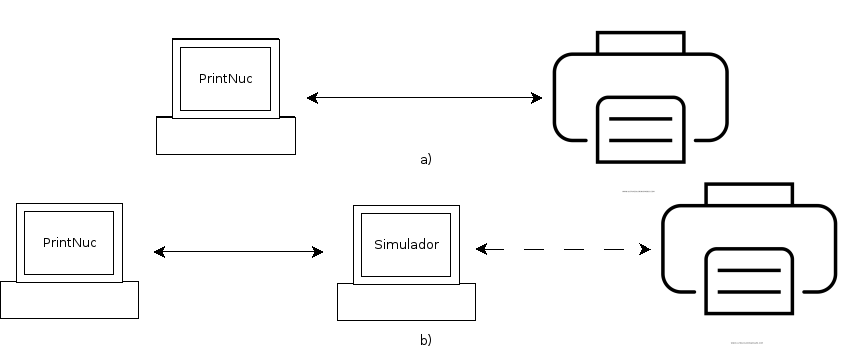
\includegraphics[width=0.8\textwidth]{img/diagrama_plc}
\caption{\label{plc_diagrama}En la imagen a) se ve como hacen pruebas actualmente con la aplicación comunicándose directamente con el \emph{PLC} directamente, por contra en la opción b), que es la solución que se da, con la opción de conectar al \emph{PLC} o no.}
\end{center}
\end{figure}

En todas estas herramientas y aplicaciones se sustenta desarrollo de la aplicación. Se ha hecho uso de nombres ficticios para conservar el anonimato de los productos de la compañía. Un ejemplo es la aplicación de la empresa la cual se conecta a la aplicación desarrollada, empleando el nombre \emph{PrintNuc} para esta aplicación a lo largo de todo el documento.

La idea que se plantea es sustituir las pruebas que se realizan entre la aplicación \emph{PrintNuc} y el \emph{PLC} de la impresora, cambiando el \emph{PLC} de la impresora por un \emph{PLC} simulado virtual. En la Figura \ref{plc_diagrama} podemos observar que la aplicación simulada también tiene como opción conectarse al \emph{PLC}, esto permite ver la información que realmente va desde \emph{PrintNuc} hasta el \emph{PLC}.

\section{Controlador lógico programable (PLC)}


Un \textbf{controlador lógico programable} o autómata programable\cite{plc_wiki}, también comúnmente denominado \textbf{PLC} por sus siglas en inglés (\textbf{P}rogrammable \textbf{L}ogic \textbf{C}ontroller), es un dispositivo empleado principalmente en la industria para automatizar procesos electromecánicos.
Los \emph{PLC} controlan la lógica a partir de procesar y recibir señales digitales y analógicas, además de poder aplicar estrategias de control.

\begin{figure}[h]
\begin{center}
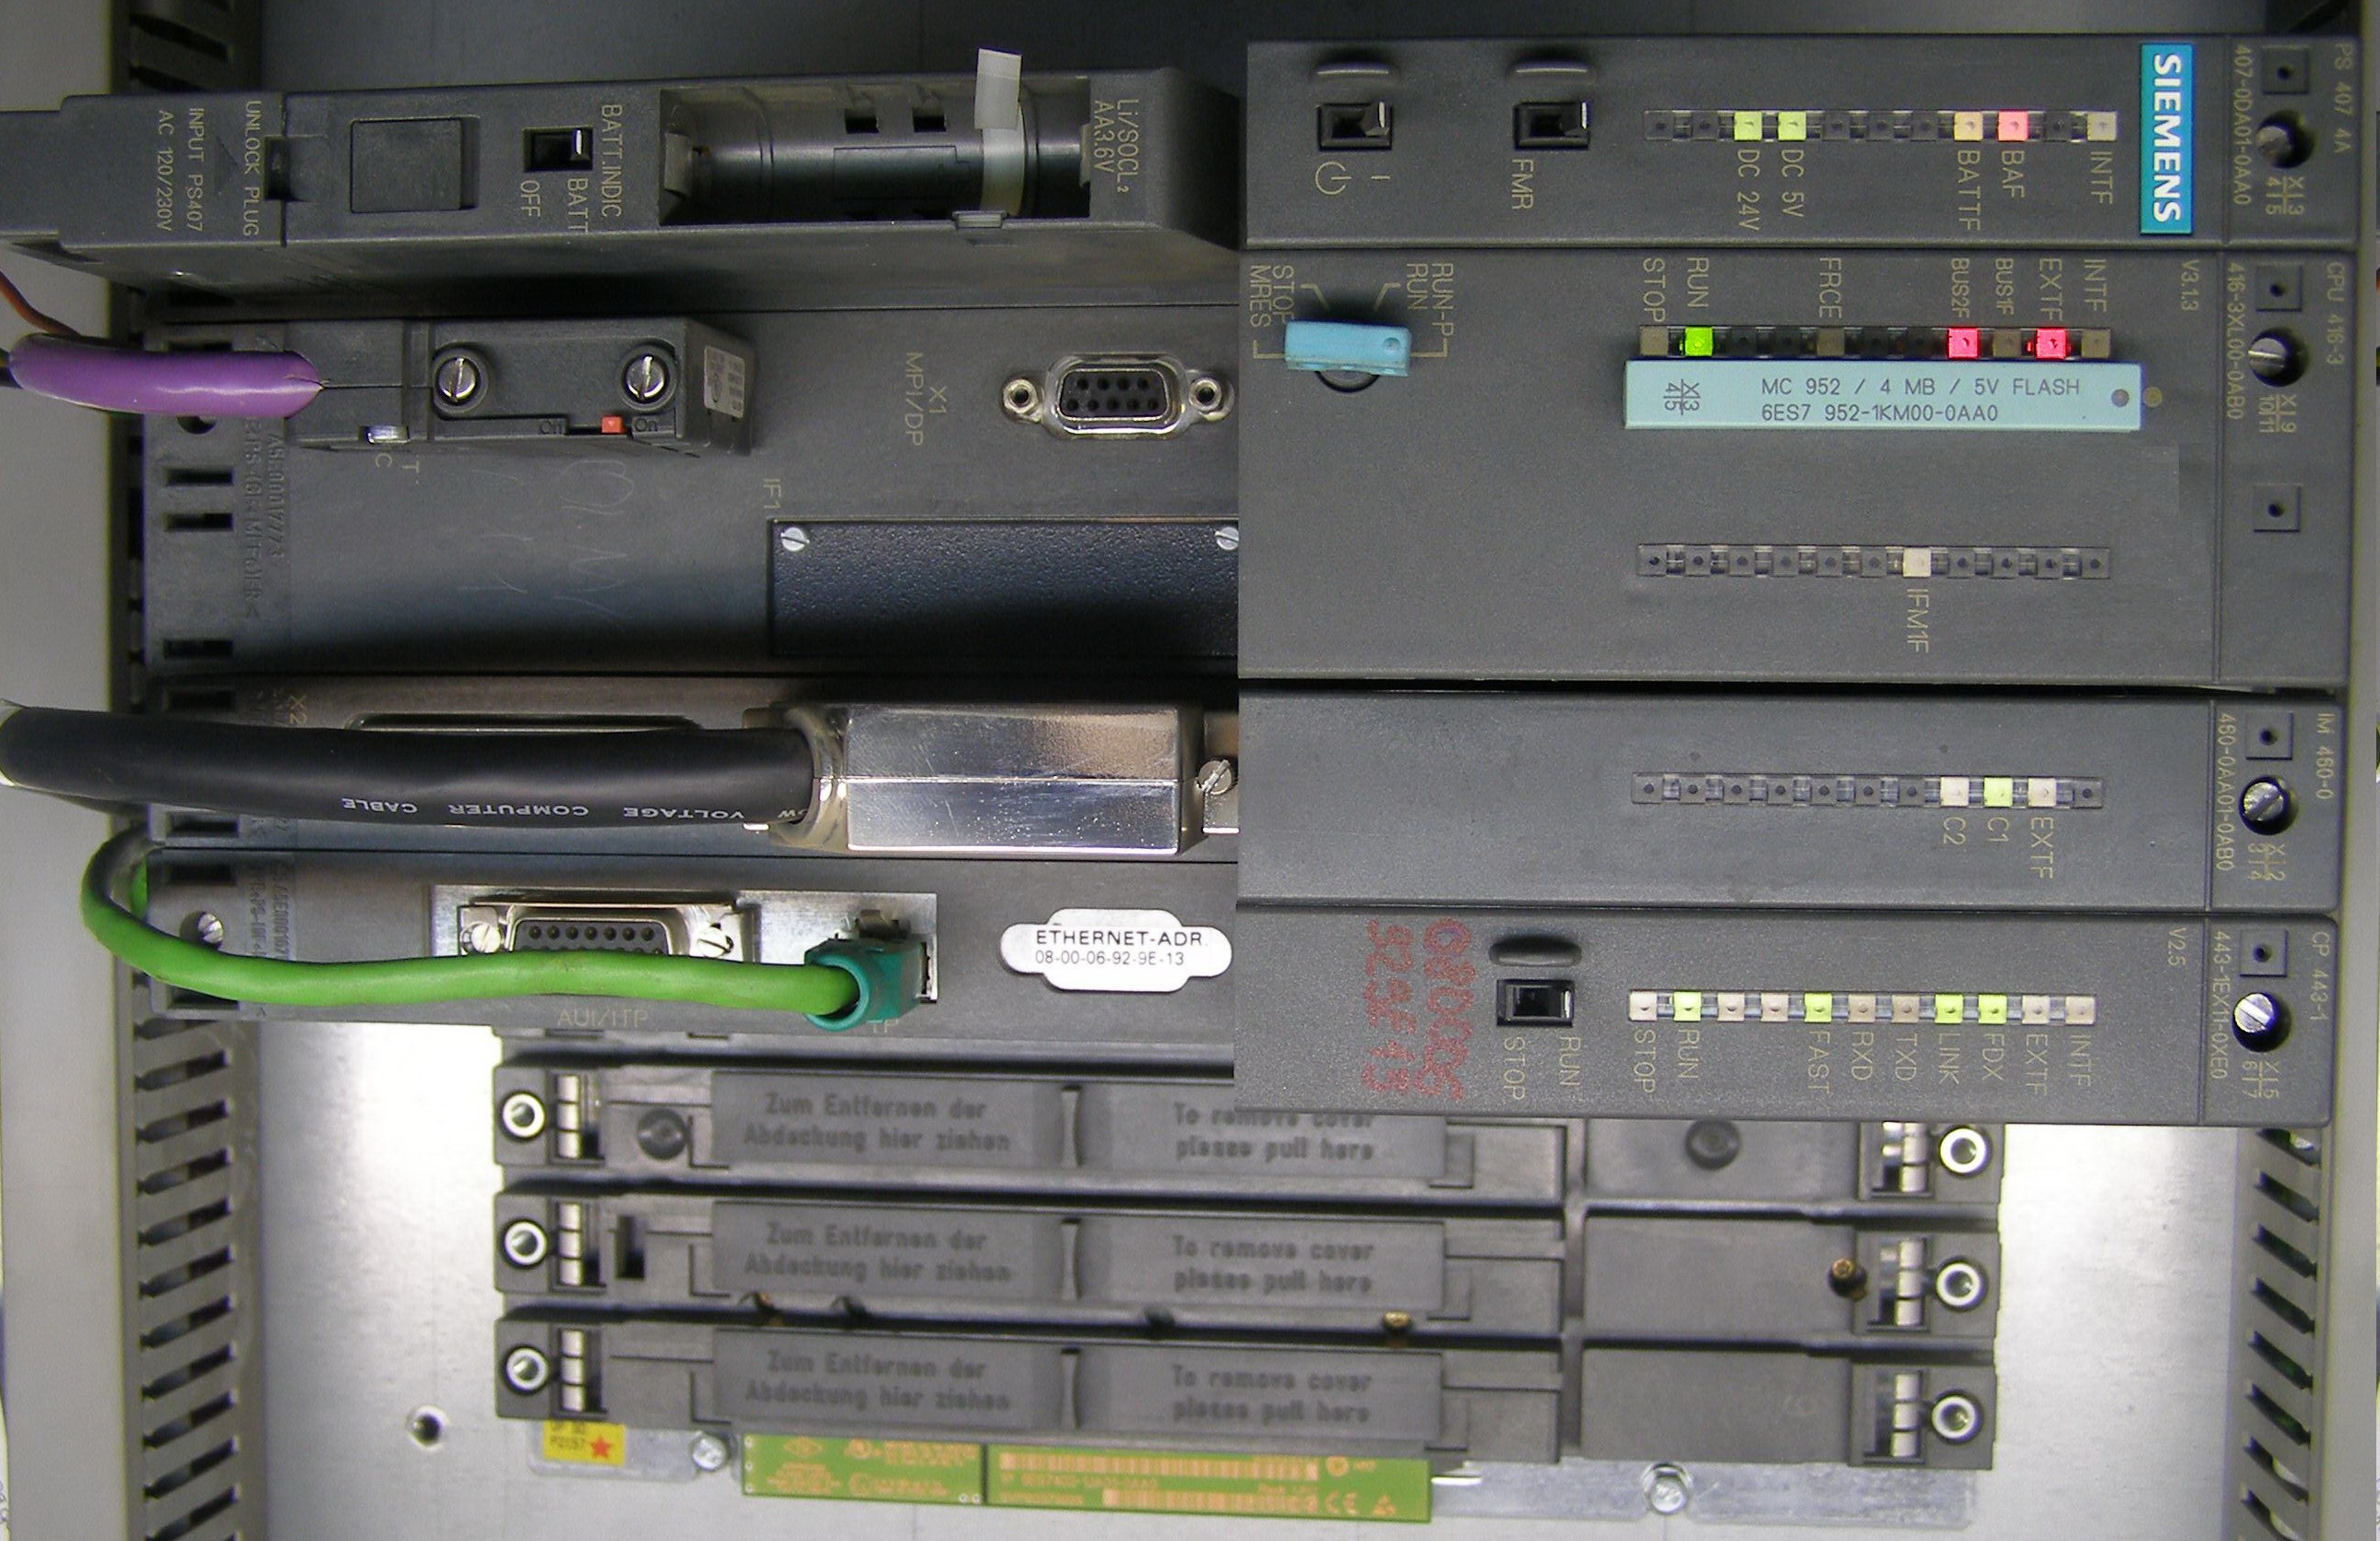
\includegraphics[width=\textwidth]{img/plc.jpg}
\caption{\label{plc_image}PLC Siemens Simatic S7-400, de arriba a abajo: fuente de alimentación, CPU, módulo de interfaz y el procesador de comunicaciones. Procedencia \textsc{Comunidad wikipedia}\cite{plc_wiki}.}
\end{center}
\end{figure}

Los \emph{PLCs} son utilizados en muchas industrias y máquinas por estar diseñados para múltiples señales de entrada y de salida, rangos de temperatura ampliados, inmunidad al ruido eléctrico y resistencia a la vibración y al impacto. Los programas para el control de funcionamiento de la máquina se suelen almacenar en baterías, copia de seguridad o en memorias no volátiles. Un \emph{PLC} es un ejemplo de un sistema de tiempo real «duro», donde los resultados de salida deben ser producidos en respuesta a las condiciones de entrada dentro de un tiempo limitado o el resultado no valdrá de nada, aún siendo correcto\cite{plc}. Podemos observar como es un \emph{PLC} en la Figura \ref{plc_image}.

\section{Metodología de trabajo Scrum}
\textbf{Scrum} \cite{scrum} es una metodología de trabajo ágil caracterizada por adoptar una estrategia de desarrollo incremental, basada en la calidad del resultado junto el conocimiento tácito de las personas en equipos autoorganizados y solapando las diferentes fases del desarrollo.

\subsection{JIRA}
\textbf{JIRA} \cite{jira} es la herramienta perteneciente a la empresa Atlassian, empleada por EFI, para poder implementar la metodología de trabajo \emph{Scrum}. Trata de ser una herramienta para la administración de tareas, el seguimiento de errores e incidencias y para la gestión operativa de proyectos.

\section{Formato de texto JSON}

\textbf{JSON} \cite{json} es un formato de texto ligero para el intercambio de datos, como \emph{XML}. Es común ver el uso de \emph{json} como sustituto de \emph{XML} o complementado junto a \emph{XML}. Destaca por la facilidad de desarrollo en analizadores y por el uso de pocos recursos empleados en las máquinas. 

\section{Microsoft Visual Studio}

\begin{figure}[h]
\begin{center}
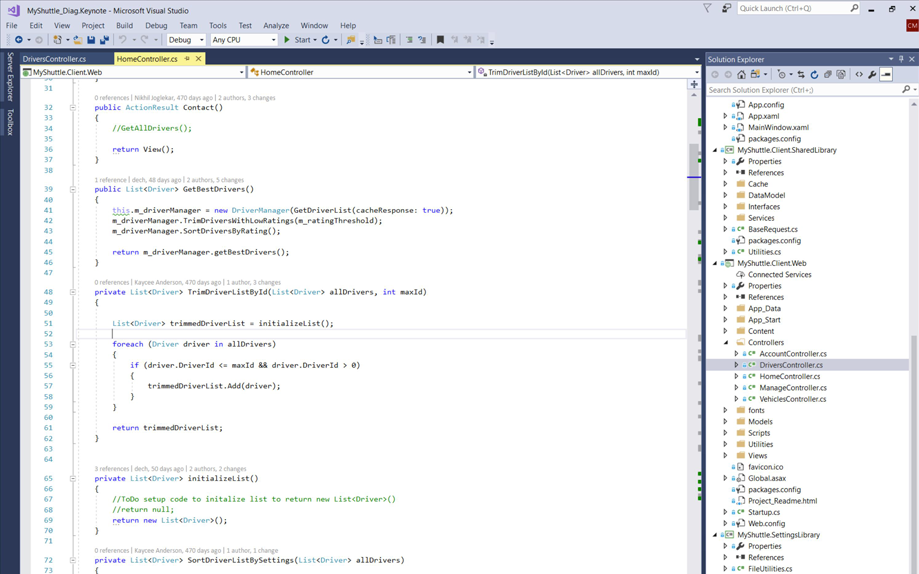
\includegraphics[width=\textwidth]{img/vs}
\caption{\label{vs}Microsoft Visual Studio en ejecución mientras se desarrolla una aplicación. Procedencia \textsc{Microsoft}\cite{visual_studio}.}
\end{center}
\end{figure}

\textbf{Microsoft Visual Studio} \cite{visual_studio} se trata de una herramienta que es un entorno de desarrollo integrado para sistemas operativos \emph{Windows}, como vemos en la Figura \ref{vs}. Soporta múltiples lenguajes de programación, entre los que destaca \textit{C\#}, por ser el empleado en el desarrollo del proyecto. Se emplea con la finalidad de escribir la aplicación, facilitando distintas tareas, como pueden ser la autocorrección, la compilación, el depurado y la inclusión de otras bibliotecas a través de un repositorio en el cual otros desarrolladores han depositado sus trabajos de forma gratuita.



\section{Lenguaje C\#}
\textbf{C\#} \cite{c_sharp} es un lenguaje de programación orientado a objetos desarrollado y estandarizado por \emph{Microsoft} como parte de su plataforma \emph{.NET}, diseñado para la infraestructura de lenguaje común.
Su sintaxis básica deriva de \emph{C/C++}, empleando el modelo de objetos de la plataforma \emph{.NET}, similar al de Java, aunque incluye mejoras derivadas de otros lenguajes como pueden ser \emph{Eiffel}, \emph{Modula-3} o \textit{Pascal}.

\section{Windows Presentation Foundation (WPF)}

\textbf{Windows Presentation Foundation (WPF)} \cite{wpf} es una tecnología de \emph{Microsoft} que permite el desarrollo de interfaces de interacción en \emph{Windows} tomando características de aplicaciones \emph{Windows}. Además ofrece una amplia infraestructura y potencia gráfica con la que es posible desarrollar aplicaciones visualmente atractivas, con facilidades de interacción, siendo fácilmente integrable con el lenguaje \emph{C\#}.

\section{Patrón Modelo-Vista-Modelo de Vista}
\textbf{El patrón modelo–vista–modelo de vista} \cite{mvvm} (en inglés, model–view–viewmodel, abreviado \textbf{MVVM}) es un patrón de arquitectura de software. Se caracteriza por tratar de desacoplar todo lo posible la interfaz de usuario de la lógica de la aplicación.
\begin{itemize}
\item El \textbf{modelo} es la capa de datos y/o la lógica de negocio, que se comunica con la aplicación para así obtener la información sin manipular  o realizar acciones directamente, además de no poder depender de la vista.

\item La \textbf{vista} representa la información a través de los elementos visuales que la componen, \textbf{siendo activas junto a comportamientos, eventos a datos} que tienen conocimiento de las capas inferiores.

\item El \textbf{modelo de vista} es la capa intermedia entre el modelo y la vista. Contiene toda la lógica de presentación, siendo estos procesos completamente ajenos a la interfaz, generando una comunicación entre la vista y el modelo de vista a través de enlaces de datos.
\end{itemize}

\section{MVVM Light Toolkit (lightmvvm)}

\textbf{MVVM Light Toolkit} \cite{mvvmlight} es una biblioteca que ayuda a reducir el tiempo de desarrollo en aplicaciones que emplean \emph{WPF}, forzando el uso del patrón \emph{MVVM} para el desarrollo de la interfaz visual, separando la interfaz (capa vista) del resto de la aplicación (capa modelo), creando una aplicación con un código mucho más legible a través de una capa intermedia (modelo de vista) mejorando el posterior mantenimiento de la aplicación.


\section{Git}

\textbf{Git} \cite{git} es un software de control de versiones pensando en la eficiencia y la fiabilidad del mantenimiento de versiones de aplicaciones cuando éstas tienen un gran número de archivos de código fuente y/o equipos de desarrollo. Su propósito es llevar el registro de los cambios en archivos de computadora y coordinar el trabajo que varias personas realizan sobre archivos compartidos a través de las ramas de trabajo que dispone.

El desarrollo de \emph{git} se realiza a través del uso de \textbf{ramas}, donde cada rama es un espacio de trabajo donde se realiza una parte del trabajo que posteriormente se juntará con otra rama para completar entre varias ramas una tarea propuesta.

Cada vez que se abre una nueva rama, normalmente se hace una copia de la rama en la que se encuentra actualmente para realizar cambios que no afectan de la rama heredada. Normalmente cuando se cierra una rama, se indica a qué rama han de afectar esos cambios, pues de otra forma, todo el trabajo realizado se perdería.

\subsection{Git-flow}

\textbf{Git-flow} es una extensión que añade comandos a \textit{git} para simplificar la gestión de ramas empleando la metodología de trabajo \textit{Scrum}. Cuando se inicia un nuevo proyecto, nos encontramos con dos ramas principales, \emph{master} y \emph{develop}, creadas inicialmente por defecto, las cuales irán sufriendo cambios haciendo uso de las ramas \emph{feature}, \emph{release} y \emph{hotfix}, teniendo cada una un uso distinto. A continuación describiremos la utilidad de cada rama:

\begin{itemize}
\item La rama \textbf{master} es la que contiene la última versión del proyecto que está en producción. Esta rama no se modifica directamente.

\item La rama \textbf{develop} contiene el último estado del programa que se está desarrollando actualmente, siendo modificada principalmente por los resultados de las ramas \emph{feature}. Esta rama no se modifica directamente.

\item Las ramas \textbf{feature} se usan para desarrollar nuevas funcionalidades, parten de la rama \textit{develop}. Cuando se cierra una rama, se fusiona otra vez con \textit{develop}.

\item Las ramas \textbf{release} se usan para lanzar una versión de producción, empleándose para realizar los cambios que sean necesarios para liberar la nueva versión, como cambios de configuración o de versión. Esta rama se crea a partir de la rama \textit{develop}, una vez se cierra, es fusionada con las ramas \textit{master} y \textit{develop}.

\item Las ramas \textbf{hotfix} se usan para cambios rápidos, con carácter urgente para solucionar problemas graves que requieren inmediatez de la rama de producción, requiriendo el arreglo de dicho fallo lo antes posible. Esta rama se crea a partir de la rama \textit{master}, una vez se cierra, es fusionada con las ramas \textit{master} y \textit{develop}.
\end{itemize}

\section{Protocolo modbus/TCP}

\textbf{Modbus}  \cite{modbus} es un protocolo de comunicaciones basado en la arquitectura maestro-esclavo, diseñado para controladores lógicos programables (\emph{PLCs}). Convertido en un protocolo de comunicaciones estándar de facto en la industria. Es el que goza de mayor disponibilidad para la conexión de dispositivos electrónicos industriales. En el desarrollo vamos a emplear \emph{modbus/TCP} ya que el despliegue de la aplicación va a realizarse sobre redes \emph{ethernet}.

En el caso de usar el protocolo \emph{modbus/TCP} se emplea la estructura cliente-servidor donde el cliente es el maestro y el servidor es el esclavo. Este punto suele ser confuso, ya que cuando se hace el cambio de la nomenclatura se suele cruzar el concepto.

\subsection{Modelo de Datos Modbus}

El \textbf{modelo de datos en modbus} distingue entre entradas digitales, salidas digitales (también denominadas \textit{coils}), registros de entrada y registros de retención (también denominados \textit{holding registers}). Las entradas y salidas digitales ocupan un bit, mientras que los registros ocupan 16 bits o 2 bytes, pudiéndose ver en el Cuadro \ref{mobdus_tamanyo} esta información.


\begin{table}[htbp]
\begin{center}
\begin{tabular}{|lcc|}
\hline
	\textbf{Tipo de objeto} & \textbf{Acceso} & \textbf{Tamaño} \\
	Entrada digital & Lectura & 1 bit \\
	Coil & Lectura/Escritura & 1 bit \\
	Registro de entrada & Lectura & 16 bits \\
	Holding registers & Lectura/Escritura & 16 bits \\
\hline


\end{tabular}
\caption{Tipos de objetos proporcionados por un dispositivo esclavo \emph{modbus} a un dispositivo maestro \emph{modbus}.}
\label{mobdus_tamanyo}
\end{center}
\end{table}

\subsection{Formato de la trama}

En el Cuadro \ref{mobdus_trama} se muestra el estándar de la trama \emph{modbus} que emplean en la comunicación el cliente y el servidor. Cabe destacar que el orden de bytes es \emph{big-endian}.

\begin{table}[htbp]
\begin{center}
\begin{tabular}{|lc p{8cm}|}
\hline
	\textbf{Nombre} & \textbf{Longitud (Bytes)} & \textbf{Función} \\
	ID de la transacción & 2 &	Sincronización entre mensajes de servidor y cliente \\
	ID del protocolo &	2 &	0 para \emph{modbus/TCP} \\
	Campo de longitud &	2 &	Número de bytes en esta trama \\
	Identificador de unidad &	1 &	Dirección del esclavo (255 si no se usa) \\
	Código de función &	1 &	Códigos de función como en otras variantes \\
	Bytes de datos &	n &	Datos como respuesta o comandos\\
\hline


\end{tabular}
\caption{\label{mobdus_trama}Visualización del formato estándar de trama \emph{modbus/TCP}.}

\end{center}
\end{table}

Se ha de comentar que el campo \emph{identificador de unidad} se utiliza con dispositivos \emph{modbus/TCP} que están compuestos por varios dispositivos \emph{modbus} en las pasarelas \emph{modbus/TCP} a \emph{modbus/RTU}. Cuando se emplea de esta forma, el identificador de unidad indica la dirección de esclavo del dispositivo detrás de la pasarela. Aún así, en muchas ocasiones los dispositivos compatibles con \emph{modbus/TCP} ignoran el identificador de unidad.

\subsection{Biblioteca NModbus4}

\textbf{NModbus4} \cite{nmodbusapi} es una biblioteca que implementa el protocolo \emph{modbus} en el lenguaje de programación \emph{C\#}. Dispone de la comunicación en distintos medios, siendo \emph{modbus/TCP} de nuestro interés, pudiéndose emplear tanto si queremos implementar un servidor o esclavo, o para implementar un cliente o maestro.

Esta biblioteca no solo ofrece soporte a la comunicación \emph{modbus}. Además también ofrece un sistema de almacenamiento para la información de la comunicación en el caso de usar la biblioteca con el fin de crear un servidor \emph{modbus}, pudiendo leer y escribir en cualquier posición del almacenamiento. 
Se ha de hacer hincapié en que el apartado de cliente o maestro no requiere utilizar el sistema de almacenamiento, puesto que solo es necesario para el servidor o esclavo, ya que necesitan un lugar donde almacenar la información que recibe. 

\section{Aplicación Modbus PLC Simulator}

\begin{figure}[h]
\begin{center}
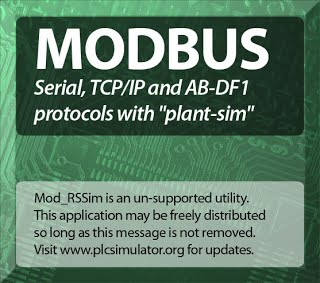
\includegraphics[width=2in]{img/ModbusPLCSimulatorNewartwork.jpg}
\caption{\label{plc_mod}Icono de la aplicación \emph{Modbus PLC Simulator}, antes llamada \emph{Mod\_RSSim}. Procedencia \textsc{Modbus PLC Simulator}\cite{plcsimulator}.}
\end{center}
\end{figure}

La aplicación \textbf{Modbus PLC Simulator} \cite{plcsimulator} ha ayudado mucho en la labor de puesta en marcha de la aplicación, ya que como bien indica su nombre y su icono que vemos en la Figura \ref{plc_mod}, realiza las labores de simulación de un servidor \emph{modbus}. Esta aplicación ha sido necesaria ya que en ningún momento se ha tenido acceso a ningún \emph{PLC}.

\begin{figure}[h]
\begin{center}
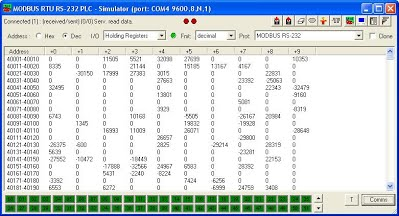
\includegraphics[width=\textwidth]{img/ModbusPLCSimulatorRegistersscreen.jpg}
\caption{\label{plc_sim}\emph{Modbus PLC Simulator} en funcionamiento. Procedencia \textsc{Modbus PLC Simulator}\cite{plcsimulator}.}
\end{center}
\end{figure}

Presentando esta aplicación, el lector puede llegar a pensar que con el uso de esta aplicación no hubiese hecho falta la necesidad del proyecto, respecto a esa idea, se puede ver en la Figura \ref{plc_sim} una muestra caótica de la representación de los datos, queriendo evitar esto con la aplicación que se ha propuesto desarrollar, aportando una interfaz mucho más amigable, sencilla y útil respecto a \emph{Modbus PLC Simulator}.

\section{Aplicación cliente Modbus}
\begin{figure}[H]
\begin{center}
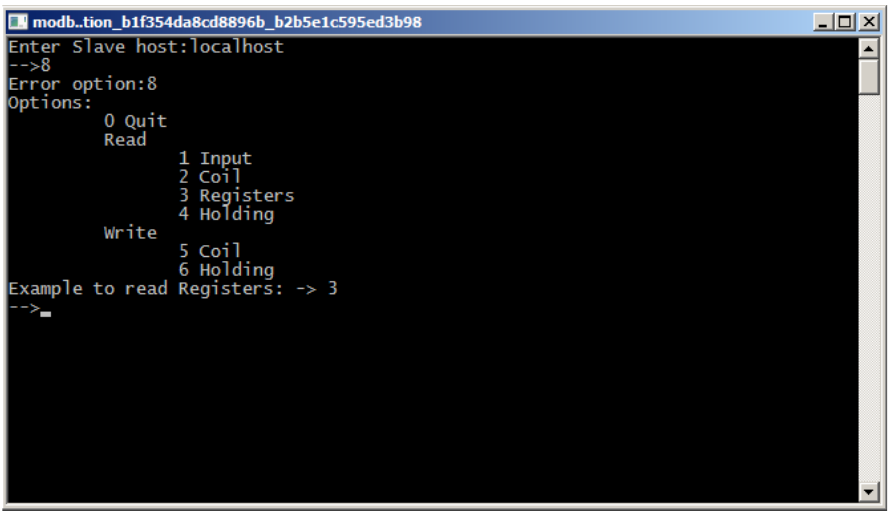
\includegraphics[width=\textwidth]{img/cliente_modbus.png}
\caption{\label{plc_cli}Aquí se visualiza el funcionamiento del cliente \emph{modbus}.}
\end{center}
\end{figure}

Esta aplicación es de desarrollo propio, realizada los primeros días de estancia en la empresa para comprobar los conocimientos obtenidos acerca del patrón \emph{MVVM} y del protocolo \emph{modbus}. Ha sido de utilidad para la puesta en marcha, puesto que en un principio no se tenía acceso a la aplicación que la compañía ofreció posteriormente para la puesta en marcha, empleándola para las comunicaciones \emph{modbus}. Como se observa en la Figura \ref{plc_cli} es una aplicación sencilla que funciona mediante consola.

\section{Wireshark}

\textbf{Wireshark} \cite{wireshark} es una aplicación que actúa sobre las redes de comunicación para realizar un análisis de los protocolos que circulan en el momento que la aplicación está conectada.


\begin{figure}[h]
\begin{center}
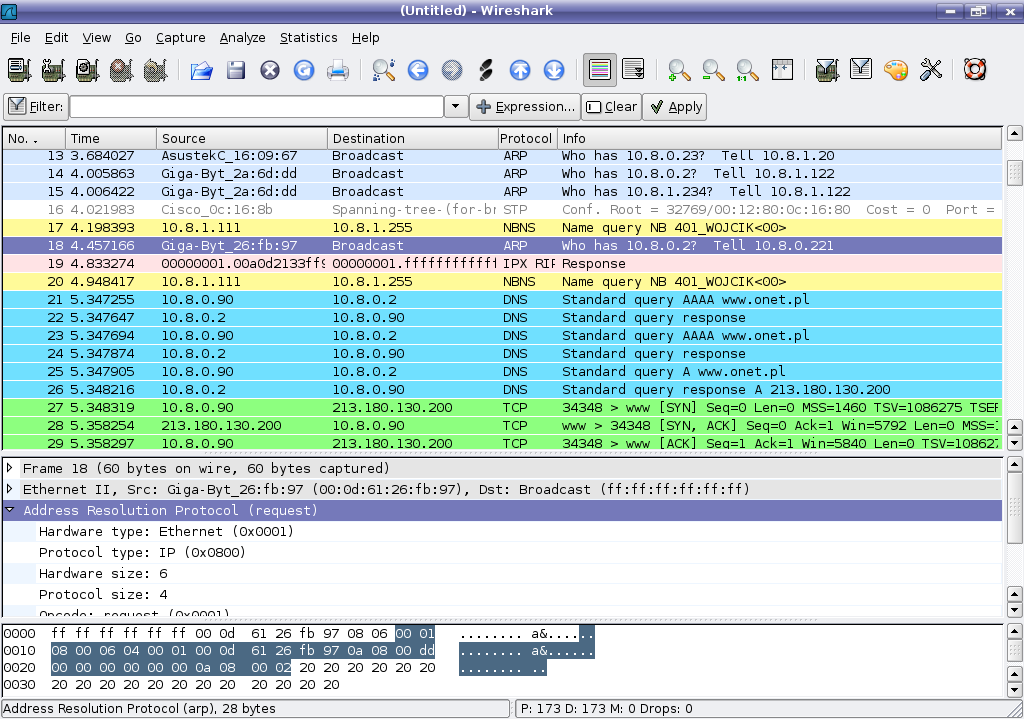
\includegraphics[width=\textwidth]{img/wireshark}
\caption{\label{vireshark}Wireshark mientras captura paquetes. Procedencia \textsc{Wireshark}\cite{wireshark}.}
\end{center}
\end{figure}

Ofrece una funcionalidad semejante al comando \emph{tcpdump}, con la intuición que da una interfaz gráfica, permitiendo mostrar todo el tráfico que pasa a través de una red, además de ayudar con opciones de organización y filtrado de información. También permite examinar datos de una red, incluso desde un archivo de captura almacenado.

Esta aplicación se usa para analizar que el tráfico que se transmite entre el maestro y el esclavo con el protocolo \emph{modbus} es el esperado, puesto que supone de gran ayuda poder filtrar el tráfico solo a paquetes \emph{modbus}, ya que suelen ser una minoría de todos los paquetes que recibe el ordenador.

\chapter{Planificación del proyecto}



\section{Metodología}
El departamento de software de EFI-Cretaprint emplea una metodología \emph{Scrum} basada en tareas a través de la plataforma \emph{JIRA}. El responsable del departamento es quien establece una tarea dentro de la plataforma y los propios desarrolladores la evalúan para que posteriormente asignen las horas de trabajo requeridas para esa tarea. Cabe decir que los propios desarrolladores también son capaces de generar subtareas a partir de las tareas. En caso de que la tarea sea muy compleja o requiera más de una semana de trabajo, se dividirá el trabajo entre los trabajadores, disminuyendo también el tiempo requerido para la tarea. La misma metodología de trabajo empleada por la empresa, va a ser la metodología empleada en el simulador de una forma mucho más informal, al tratarse de un producto interno del departamento y no seguir las líneas generales de desarrollo de la empresa.

\section{Requisitos}
%\textbf{Requisitos técnicos y materiales.}

Los requisitos especificados por la empresa no han sido muy concretos, puesto que el principal ha sido el uso de los mismos recursos y herramientas que emplea la empresa, pudiéndose ver parte de las herramientas utilizadas en el capítulo 2. Otros de los recursos necesitados para la elaboración del proyecto han sido un ordenador de sobremesa, con sus respectivos periféricos, que sea capaz de soportar el funcionamiento de las aplicaciones y conexión a internet para poder acceder a los recursos de la empresa y de terceros.

\section{Planificación}

\subsection{Planificación inicial}

\begin{figure}[H]
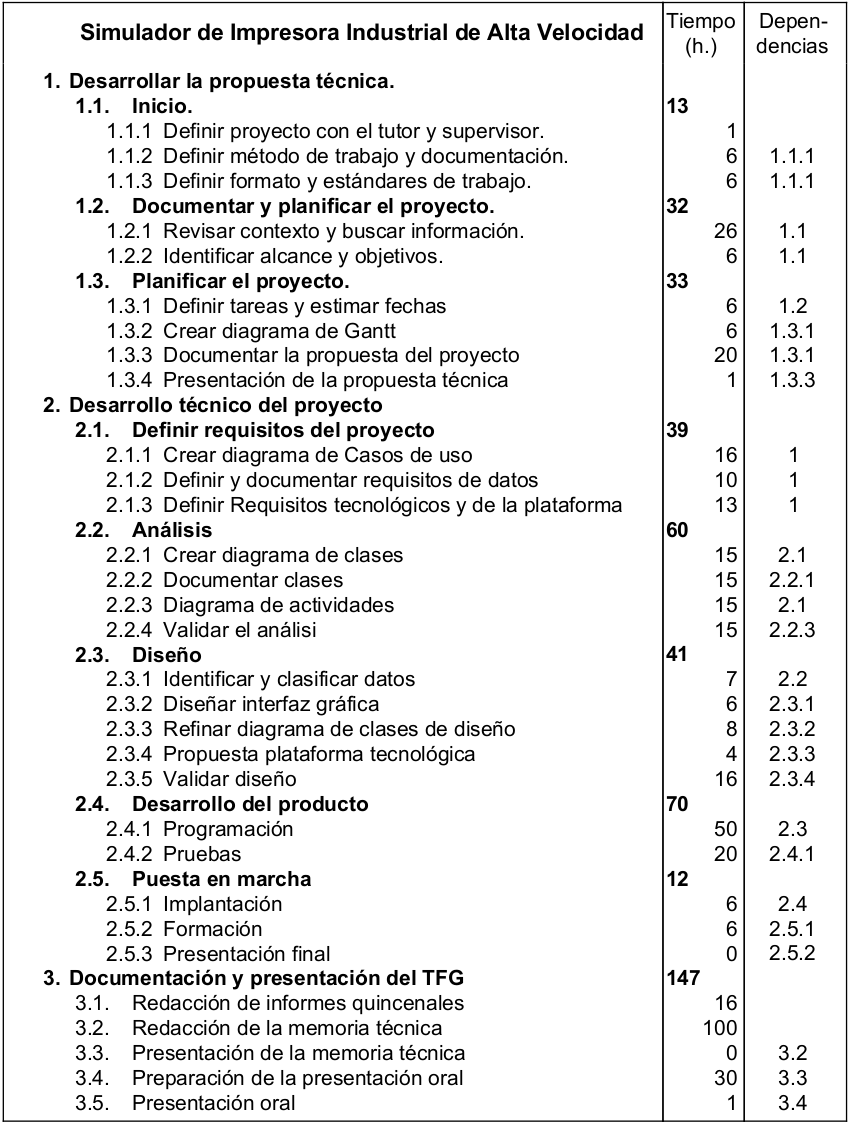
\includegraphics[width=0.93\textwidth]{img/lista_tareas.png}
\caption{\label{tareas_inicial}Desglose en tareas, junto con la planificación temporal y las dependencias entre tareas de la planificación inicial.}
\end{figure}

\subsection{Planificación final}

\begin{figure}[H]
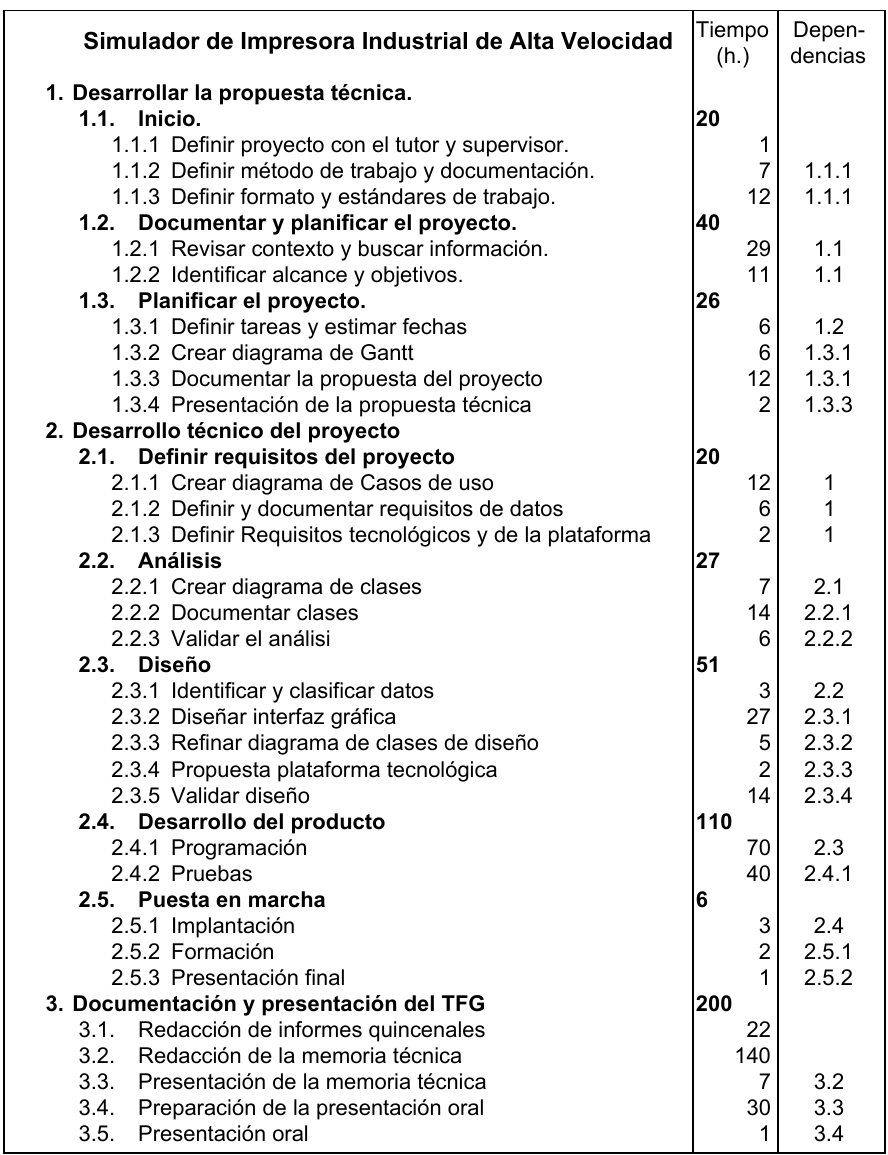
\includegraphics[width=0.97\textwidth]{img/lista_tareas_final.png}
\caption{\label{tareas_final}Desglose en tareas, junto con la planificación temporal y las dependencias entre tareas de la planificación final.}
\end{figure}

\subsection{Diagrama de Gantt inicial}

\begin{figure}[H]
\begin{center}
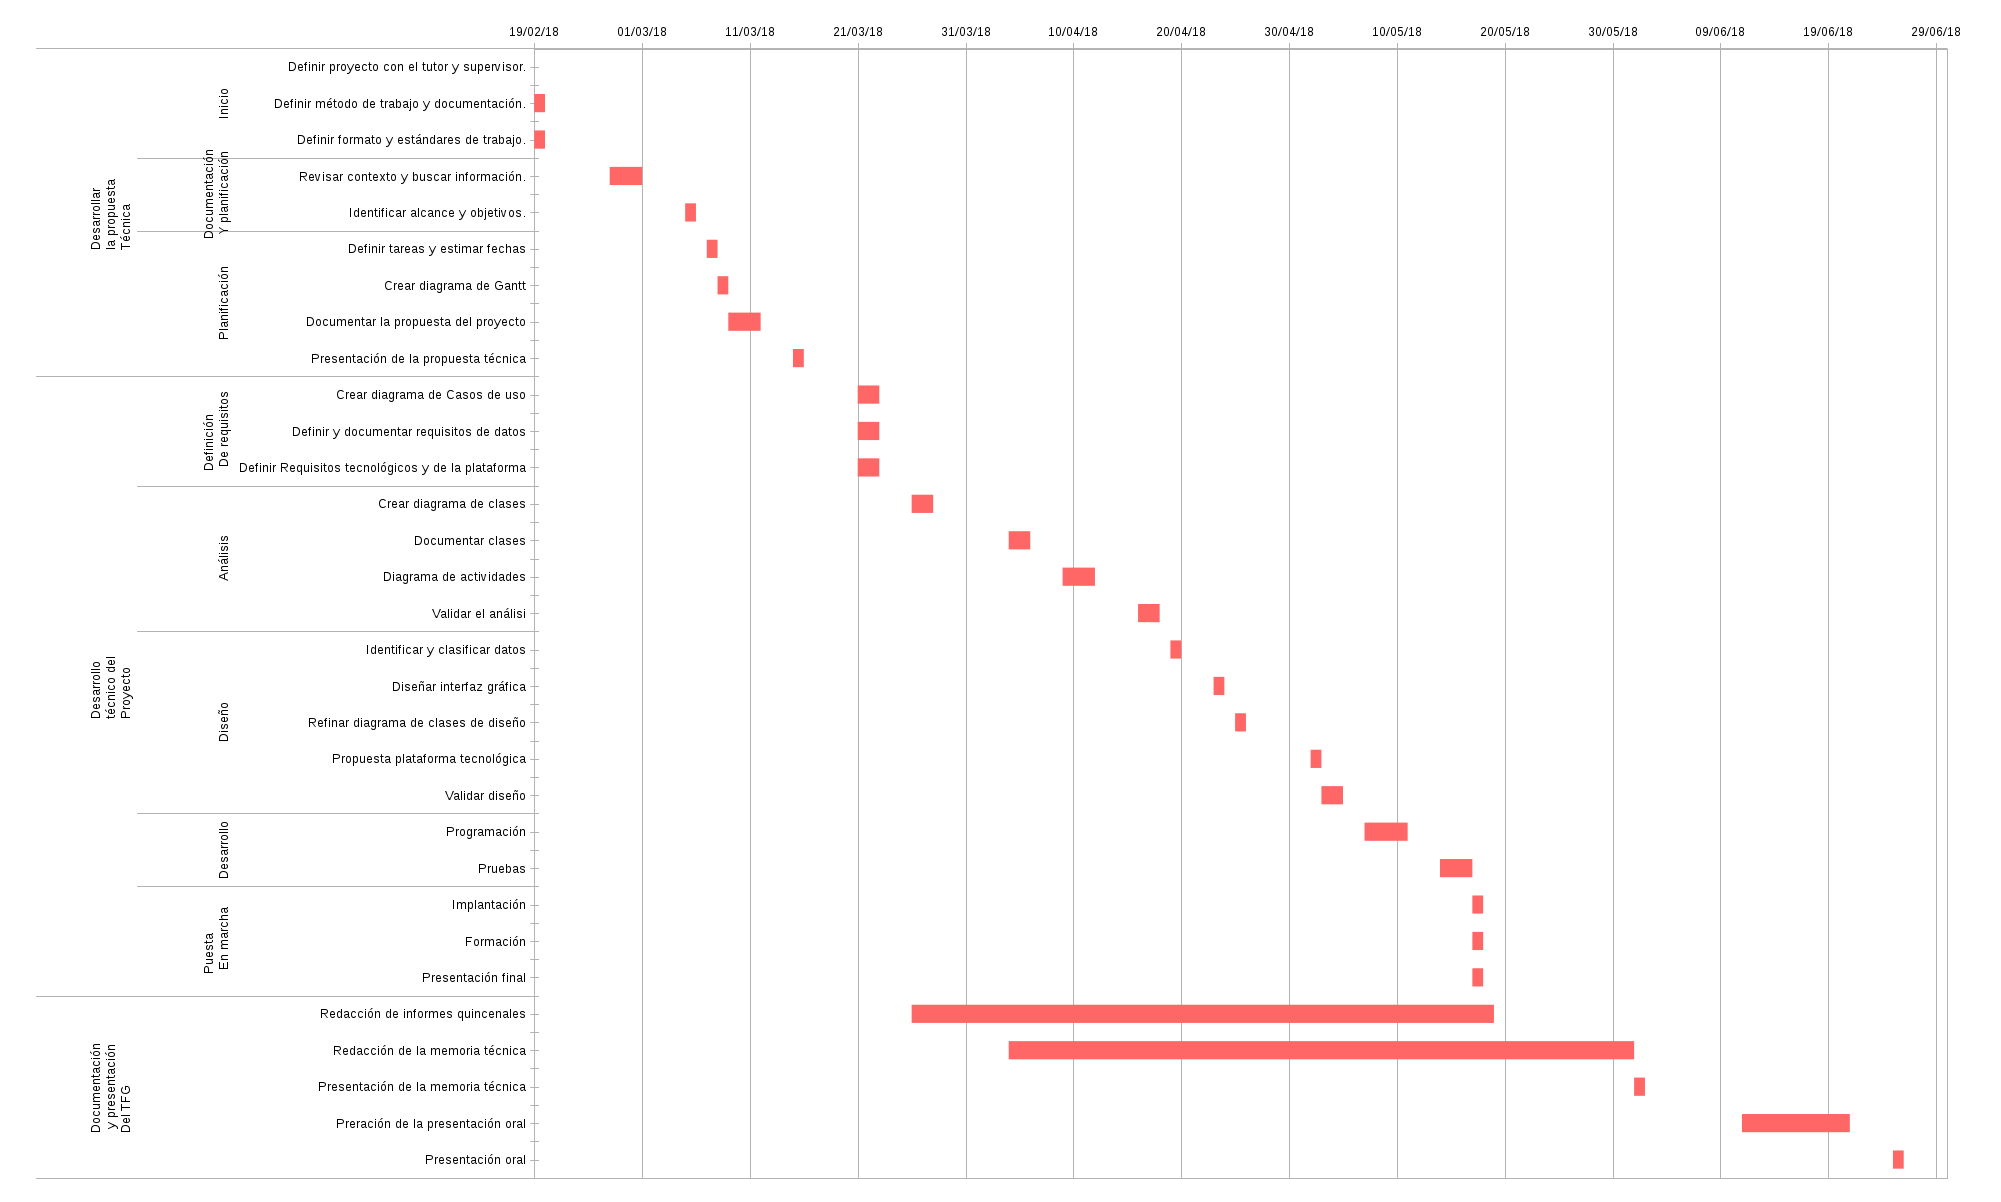
\includegraphics[angle=90,width=0.78\textwidth]{img/diagrama_gantt.png}
\caption{\label{gantt_inicial}Diagrama de Gantt inicial indicando por días la división del trabajo.}
\end{center}
\end{figure}

\subsection{Diagrama de Gantt final}

\begin{figure}[H]
\begin{center}
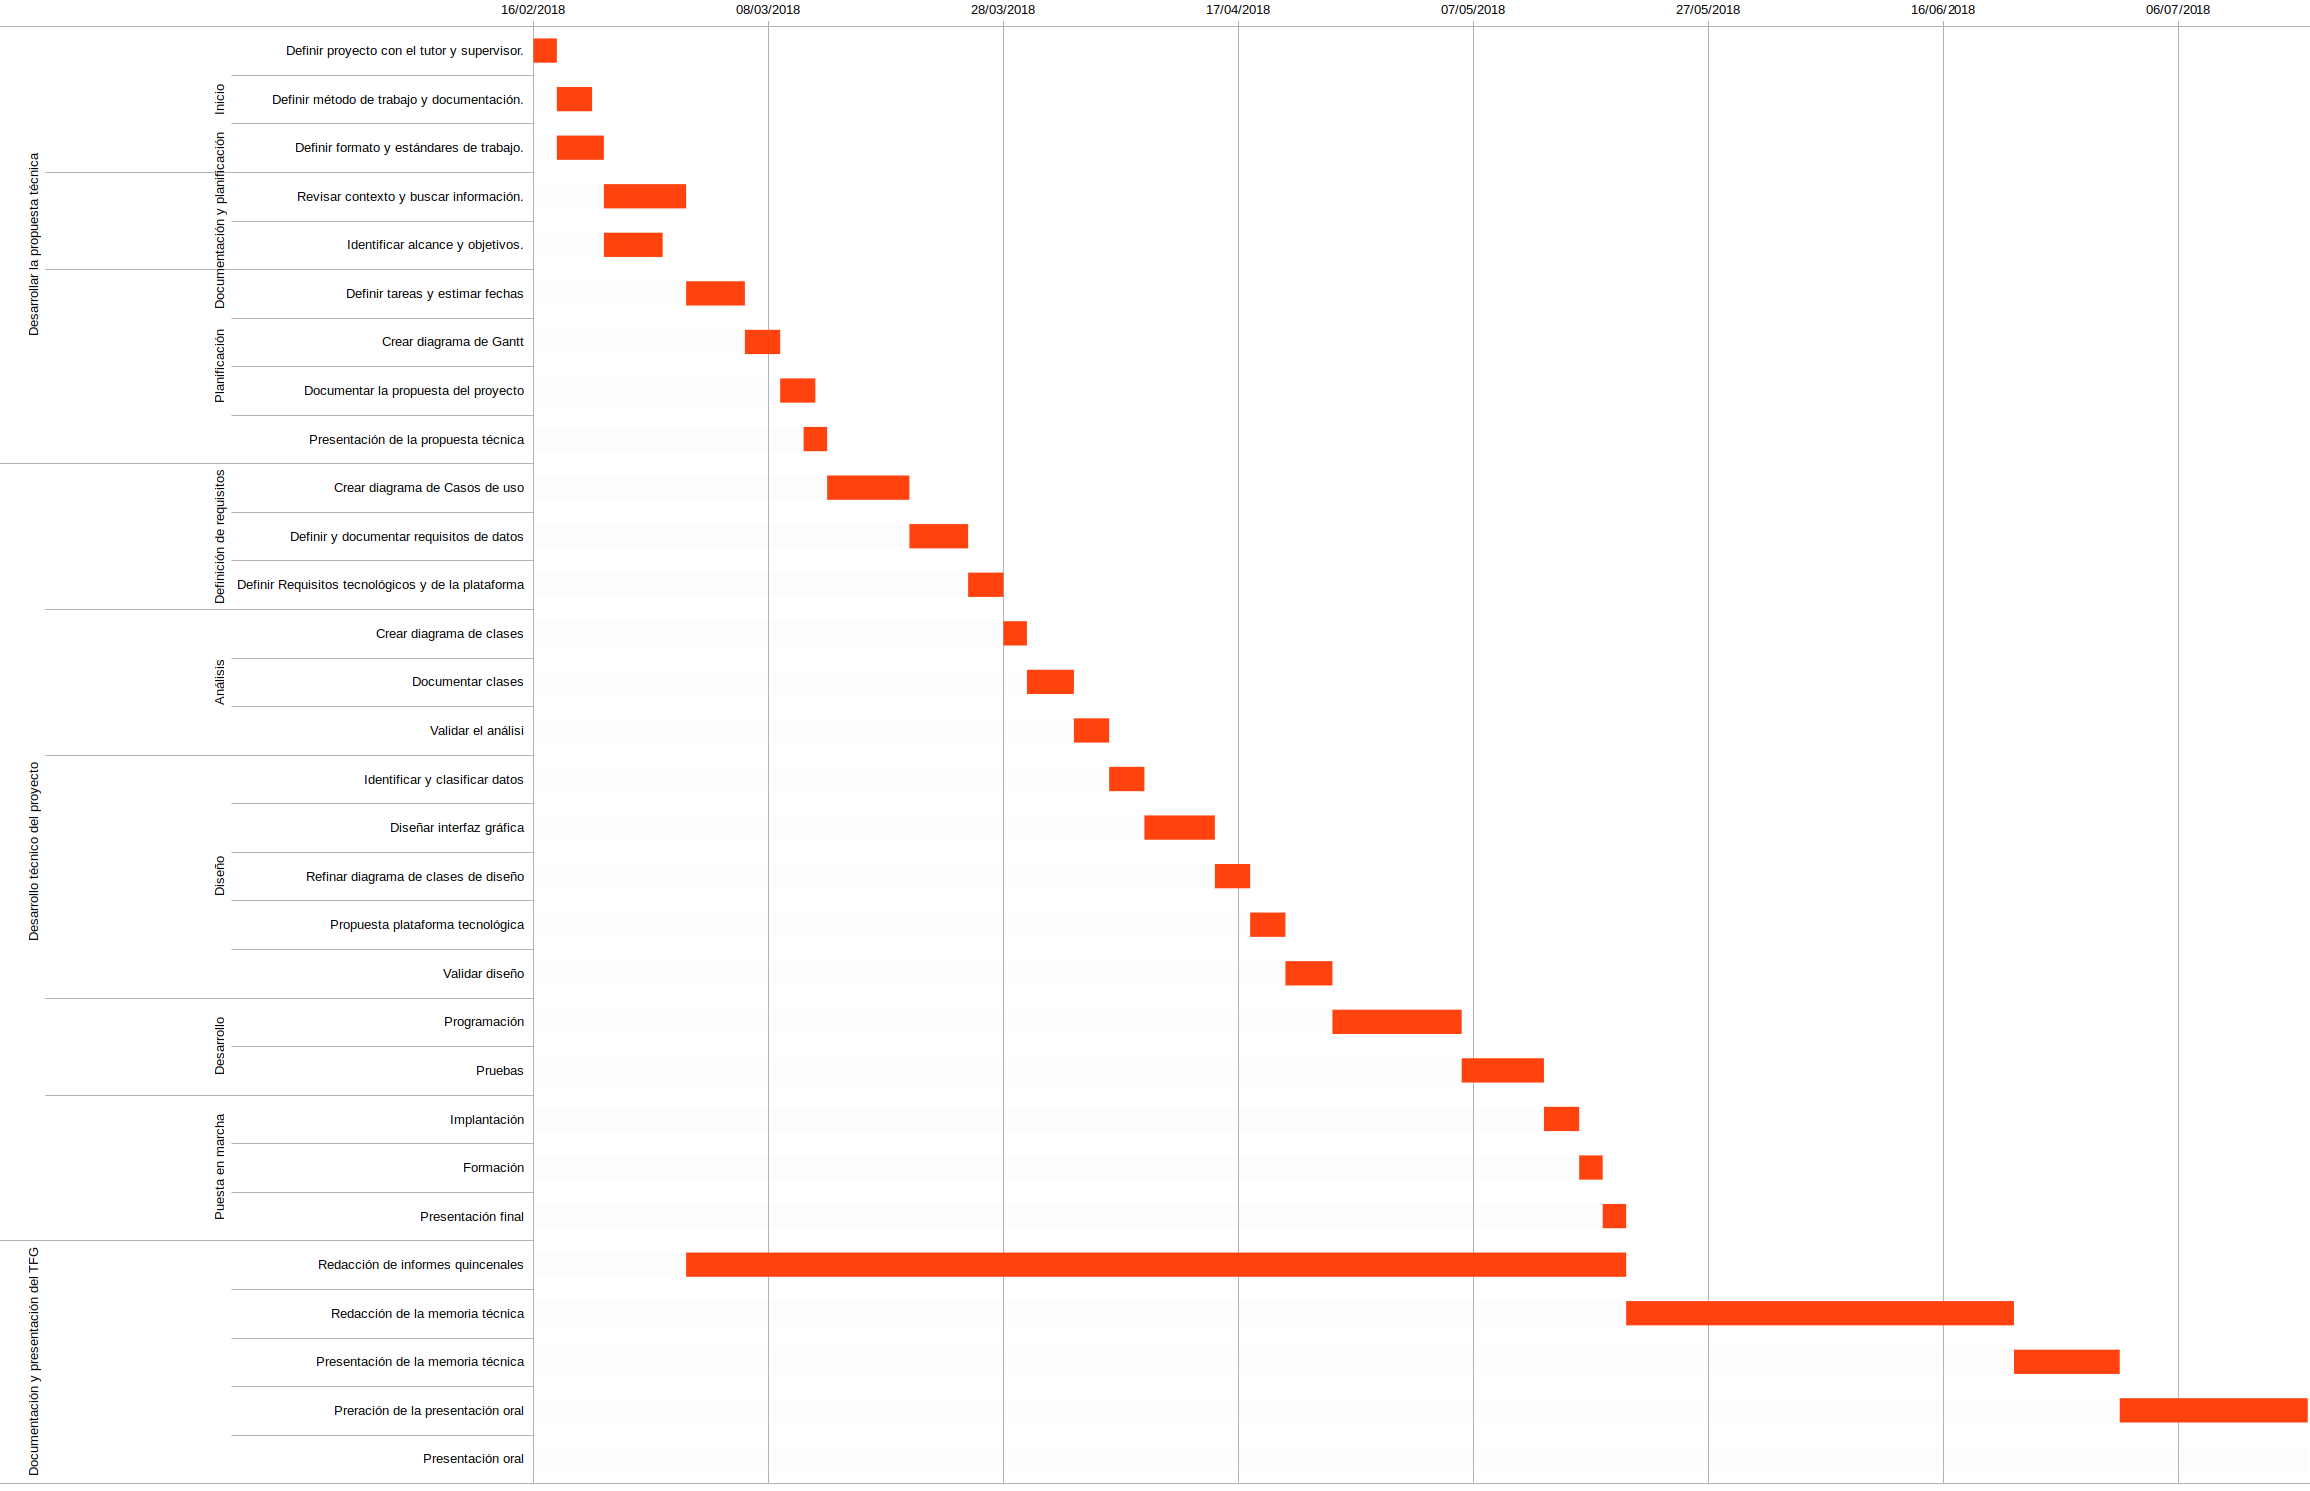
\includegraphics[angle=90,width=0.84\textwidth]{img/gantt_final.png}
\caption{\label{gantt_final}Diagrama de Gantt final indicando por días la división del trabajo.}
\end{center}
\end{figure}

\subsection{Diferencias entre la planificación inicial y la planificación final}

La planificación inicial del proyecto, tal como se puede ver en la Figura \ref{tareas_inicial} ha sido bastante acertada al número de horas realizadas en cada tarea respecto a la planificación final que se muestra en la Figura \ref{tareas_final} a pesar de los contratiempos ocurridos. Esto ha sido posible gracias a incluir en los ciertos puntos del proyecto que se consideraban críticos una mayor cantidad de horas respecto a otros puntos. En el diagrama de Gantt de la Figura \ref{gantt_inicial} se puede observar el número inicial de horas que se iba a emplear para cada tarea. Por contra, se nota claramente un incremento de horas en determinadas tareas y reducción en otras tareas como se muestra en el diagrama de Gantt final de la Figura \ref{gantt_final}.

\section{Estimación de recursos y coste del proyecto}

Los recursos necesarios para desarrollar el proyecto han sido solamente aplicaciones de terceros o de la empresa de carácter gratuito, evitando así el coste económico por este proyecto. Por contra vamos a explicar cual seria el coste estimado del proyecto si hubiese que desarrollarlo partiendo de cero. Dos puntos que se han de aclarar para no dar confusiones son el coste de ciertos materiales, como puede ser el ordenador y el monitor, y el salario que hubiese percibido un trabajador, en función de la tarea asignada.

El precio del ordenador\cite{pc} es de 599'00\euro \ y del monitor\cite{monitor}, 117'95\euro. Para tener el coste de estos productos durante el tiempo que se han necesitado, se ha contado con una duración de cada elemento de 60 meses. Para obtener el coste mensual se ha dividido el coste de cada producto entre 60 meses.

El cálculo del salario se basa en el salario mínimo interprofesional de un programador y un analista\cite{salario}. Se ha separado en dos tipos distintos de salarios, ya que la tarea de cada uno requiere unos conocimientos y aptitudes completamente distintos, creando diferencia entre los distintos salarios que pueda recibir uno u otro. El salario mínimo de un programador es de 1588\euro/mensuales, en cambio el de un analista es de 1924\euro/mensuales.

En el Cuadro \ref{costes} se muestran todos los materiales y servicios necesitados, junto a su precio, así como el coste total del proyecto.

\begin{table}[h]
\begin{center}
\begin{tabular}{|l|c|r|r|}
\hline
\multicolumn{1}{|c|}{\textbf{Recurso}} & \textbf{Unidades} & \multicolumn{1}{|c|}{\textbf{Coste}} & \multicolumn{1}{|c|}{\textbf{Total}} \\
\hline
Ordenador HP Pavilion Power 570-P044NS\cite{pc} (\euro/mes) & 3 & 9'98\euro & 29'95\euro  \\
\hline
Monitor Samsung S24D330\cite{monitor} (\euro/mes) & 3 & 1'97\euro  & 5'90\euro  \\
\hline
Ratón L-Link LL-2080-R\cite{raton} & 1 & 1'95\euro  & 1'95\euro  \\
\hline
Teclado Kloner KTU20\cite{teclado} & 1 & 4'95\euro  & 4'95\euro  \\
\hline
Netllar Internet 30\cite{internet} (\euro/mes) & 3 & 19'99\euro  & 59'97\euro  \\
\hline
	Salario como programador (\euro/hora) & 116 &  9'15\euro & 1061'40\euro \\
\hline
	Salario como analista (\euro/hora) & 184 &  11'08\euro & 2038'72\euro \\
\hline
	\multicolumn{3}{|c|} {Total} & 3245'59\euro \\
\hline
\end{tabular}
\caption{\label{costes}Tabla con los costes si el proyecto hubiese partido de cero.}
\end{center}
\end{table}

En coste total del proyecto partiendo de cero sería de 3245'59\euro, siendo gran parte del presupuesto la mano de obra, puesto que los elementos de los cuales se necesitan no resultan muy costosos. Por la parte software todos los programas empleados son los del capítulo 2, siendo todos ellos de uso gratuito, tanto para particulares, como para empresas.


\section{Seguimiento del proyecto}

Todas las fases del proyecto han sido supervisadas por el tutor y el supervisor mediante informes quincenales donde están descritas las tareas realizadas durante cada quincena así como los objetivos propuestos para la próxima quincena, los problemas encontrados durante el desarrollo y las tomas de decisiones ante estos problemas. Los problemas encontrados durante el desarrollo del proyecto también se encuentran explicados a lo largo de este documento, junto a una descripción de las acciones llevadas a cabo. No obstante, en la lista que aparece a continuación se encuentran las incidencias más destacadas durante el desarrollo del proyecto:

\begin{itemize}
\item La creación de eventos ante el desconocimiento de éstos. No se tiene en cuenta que fueran necesarios para el desarrollo de la aplicación.
\item Incompatibilidad entre el protocolo \emph{modbus} y la biblioteca \emph{NModbus4}. Al momento de almacenar la información, la biblioteca no almacena la información en las mismas direcciones.
\item Mala configuración de los dominios de escucha al poner en marcha el esclavo \emph{modbus}. La aplicación no se encuentra a la espera de escuchar en cualquier dirección, sólo en una en concreta.
\item Mala implementación al desarrollar la aplicación. La aplicación no funciona de forma fluida cuando recibe muchas peticiones al estar mal planteada la implementación.
\item Mala implementación del uso de la biblioteca de la empresa. No se tiene en cuenta el detalle que la biblioteca genera un desplazamiento en base 10.
\item Fallos al detener las comunicaciones bruscamente. Esta prueba se hace para comprobar como actúa la aplicación cuando una comunicación no se cierra correctamente.
\end{itemize}

\chapter{Análisis y diseño del sistema}

\section{Análisis del sistema}

El requisito principal de la aplicación es suplir el funcionamiento del \emph{PLC} de la impresora, para que no sea necesario depender de dicho componente para poder realizar pruebas. Al estar destinado al usuario técnico, se da total libertad para el diseño de la interfaz de usuario. La comunicación con el dispositivo se hace a través de cable de par trenzado empleando el protocolo \textit{mobdusTCP} mediante una red \emph{ethernet}. Además, el código se ha de realizar en \emph{C\#}, junto con las bibliotecas \emph{NModbus4}, \emph{WPF}, \emph{mvvmlight} y el protocolo interno propio que funciona sobre el protocolo \emph{modbus}.

A partir de la lista de las metas que ha de cumplir el programa a desarrollar, se muestra la siguiente lista de las acciones que se han de llevar a cabo:

\begin{itemize}
\item Comunicación del dispositivo mediante el protocolo \emph{modbus}.
\item Responder a las solicitudes, según dicta el protocolo interno de la empresa.
\item Generar posibles resultados que se asemejen lo más posible a un \emph{PLC} real.
\item Generar una interfaz para el uso del programa.
\item Comprender el programa cedido por la empresa del cual se va a partir.
\item No depender de herramientas físicas externas.
\end{itemize}

%\textbf{Posibilidad de incluir las acciones finales llevadas a cabo}
\section{Diseño de la arquitectura del sistema}

\begin{figure}
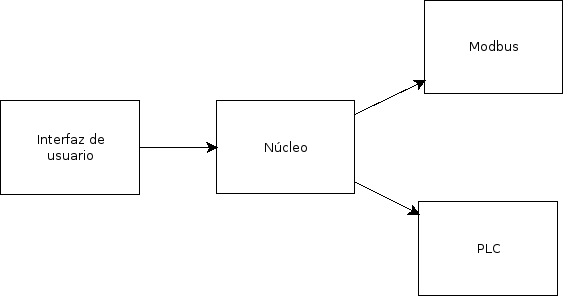
\includegraphics[width=\textwidth]{img/disenyo_arquitectura.png}
\caption{\label{disenyo_arquitectura}Dependencias entre los elementos de la aplicación.}
\end{figure}

El sistema se ha diseñado en base a 4 elementos, mostrando la relación en la Figura \ref{disenyo_arquitectura}:
\begin{itemize}
\item \textbf{Núcleo}: Es la parte que ayuda a comunicar las distintas partes del sistema.
\item \textbf{Modbus}: Es la parte que se encarga de la comunicación con otras aplicaciones.
\item \textbf{PLC}: Hereda del código de la empresa, adaptándose a las necesidades de nuestra aplicación.
\item \textbf{Interfaz de usuario}: Es la parte de la comunicación con el usuario.
\end{itemize}

\section{Diseño de la interfaz}
\begin{figure}
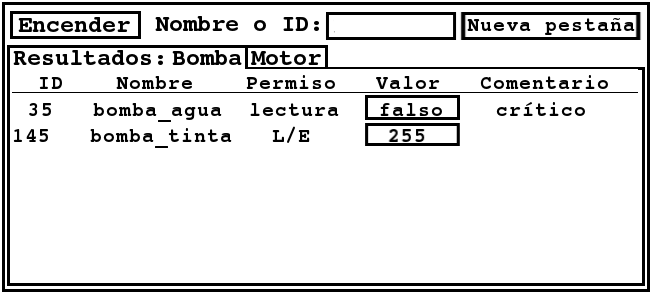
\includegraphics[width=\textwidth]{img/disenyo_ui0.png}
\caption{\label{disenyoUI0}Primer diseño de la aplicación en base a las características propuestas.}
\end{figure}


Para realizar el diseño de la interfaz se buscó que cumpliera una serie de requisitos que se vieron importantes para una aplicación enfocada a un usuario técnico. Estos requisitos para la interfaz de usuario son:

\begin{itemize}
\item Buscar por identificador o nombre los campos que se desean visualizar.
\item Separar las búsquedas en nuevas ventanas.
\item Mostrar siempre la información actualizada en la pantalla.
\item Hacer uso directo del teclado para la interacción con la aplicación.
\item Modificar los datos rápidamente.
\end{itemize}

\begin{figure}
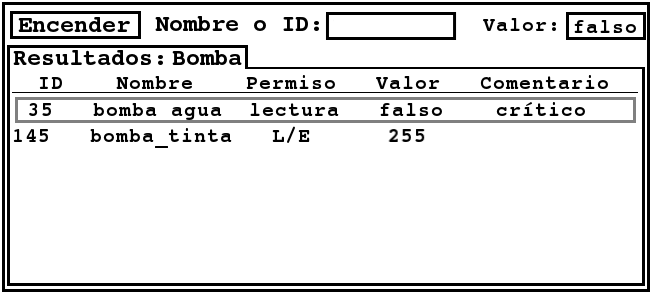
\includegraphics[width=\textwidth]{img/disenyo_ui1.png}
\caption{\label{disenyoUI1}Edición propuesta después de la complejidad de desarrollar la primera idea.}
\end{figure}

En el proceso del diseño de la interfaz se tuvo una primera idea de que el programa tuviese una interfaz visual mediante consola de comandos para el cumplimiento de los requisitos. El problema de este tipo de interfaz es la incapacidad de actualizar los cambios que ocurran durante la ejecución del programa con una sencilla implementación. Por ello, se tomó la decisión de emplear una interfaz gráfica intuitiva y sencilla, como aparece en la Figura \ref{disenyoUI0} que cumpliese con los requisitos propuestos. La interfaz permite interactuar con ella mediante: un botón para activar/desactivar la escucha del simulador mediante \emph{modbus}, una caja de búsqueda para filtrar los resultados que se muestran más abajo,y y un botón que genera una pestaña con los elementos filtrados de la caja de búsqueda.

Ante la incapacidad de poder realizar la funcionalidad que permite modificar los valores de los datos que se encuentran dentro de la lista filtrada en el tiempo establecido, se decidió hacer un cambio de la interfaz. Esto obligó a rediseñar la interfaz para que fuese posible desarrollarla en el menor tiempo posible, cambiando la opción de edición de cada línea de la lista a un campo nuevo estático en la parte superior de la aplicación, haciendo un poco más incomprensible y poco intuitiva la interfaz como se puede ver en la Figura \ref{disenyoUI1}.

El diseño presentado continuó dando problemas, aparte que se veía feo, sumado a que en la ejecución no realizaba un buen funcionamiento el programa, haciendo imposible editar los elementos por un mal diseño visual desarrollado. Este acontecimiento obligó a cambiar la forma en la que se visualiza el campo que modifica los datos de cada elemento. Esta vez se optó por separar la acción de edición de elementos en una ventana nueva, para así que no tengan relación las acciones de edición con el resto de la aplicación. Cabe destacar que en el momento que aparece esta nueva ventana, inhabilita toda acción que se pueda hacer en la ventana principal, para así evitar posibles errores de interacción.

\begin{figure}
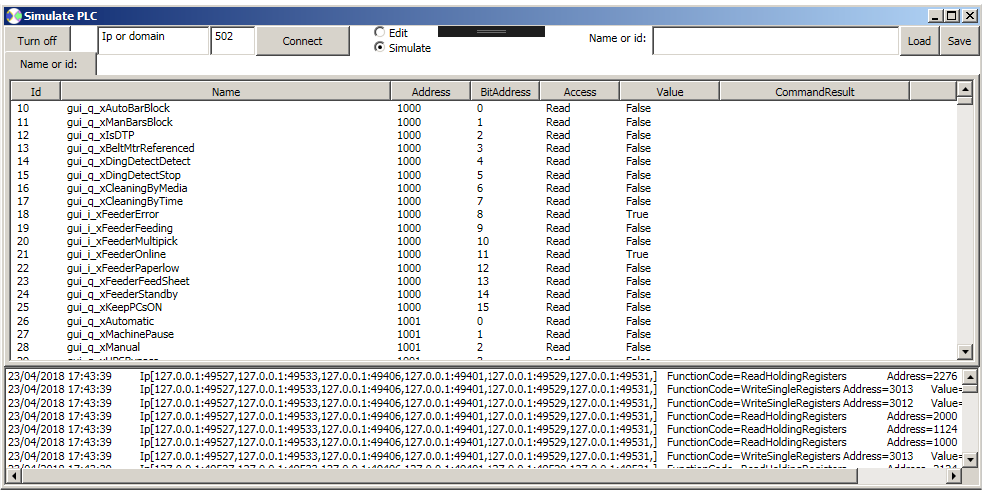
\includegraphics[width=\textwidth]{img/disenyo_ui2.png}
\caption{\label{disenyoUI2}Interfaz final de la aplicación.}
\end{figure}

Aparte de los cambios producidos por el problema de la edición de los datos, también se añadieron nuevas opciones de uso a la aplicación, así como un campo para indicar a la aplicación a qué \emph{PLC} conectarse o dos botones donde que permiten almacenar y carga la información que se encuentra en ese instante en la aplicación. También se añadió una zona donde se muestra las conexiones que recibe la aplicación, con la dirección y el motivo de la conexión, para así tener un mayor control de lo que está ocurriendo con el programa. Todos estos cambios se pueden observar en la Figura \ref{disenyoUI2} con la interfaz ya terminada.


%\begin{figure}
%\includegraphics[]{disenyo_emergente.png}
%\caption{\label{disenyo_emergente}Ventana emergente que aparece para modificar los datos.}
%\end{figure}

\chapter{Implementación y pruebas}

\section{Detalles de implementación}

En este apartado se describe cuál ha sido el paso a paso del desarrollo de la aplicación.

\subsection{Conocimiento de las tecnologías}

La primera actuación en este proyecto ha sido documentarse acerca de las tecnologías que la empresa emplea en el día a día, además de conocer las capacidades, funcionalidades, utilidad y uso que ofrecen todas estas tecnologías. La primera acción llevada a cabo ha sido aprender el patrón de diseño \emph{Modelo-Vista-Modelo de Vista} a través de la propia web de \emph{Microsoft}\cite{mvvm}. Una particularidad que tiene este patrón es que es parecido al patrón \emph{Modelo-Vista-Controlador} que enseña la universidad en los estudios del Grado. Posteriormente se ha aprendido el protocolo \emph{modbus} empleado para la comunicarse con los \emph{PLCs} por distintos medios de transmisión de datos. En concreto, se va a emplear \emph{modbus/TCP}, que es el más utilizado hoy en día por la gran cantidad de redes \emph{ethernet} que existen actualmente, consiguiendo un bajo coste de materiales. Toda la información necesaria sobre dicho protocolo puede encontrarse en su página web principal\cite{modbustcp}.

\subsection{Desarrollo de un cliente \emph{modbus/TCP}}

Para la primera toma de contacto con las tecnologías descritas en el apartado anterior, la empresa pidió que se hiciera un maestro \emph{modbus} empleando la biblioteca \emph{NModBus4}, que después se emplearía para la realización de pruebas con la aplicación final. La aplicación de prueba cuenta de una interfaz sencilla vía consola, la cual permite recibir la información del esclavo \emph{modbus}, así como también modificar las posiciones indicadas. Podemos ver las opciones de funcionamiento que da la aplicación en la Figura \ref{cliente_mod}.

\begin{figure}[h]
\begin{center}
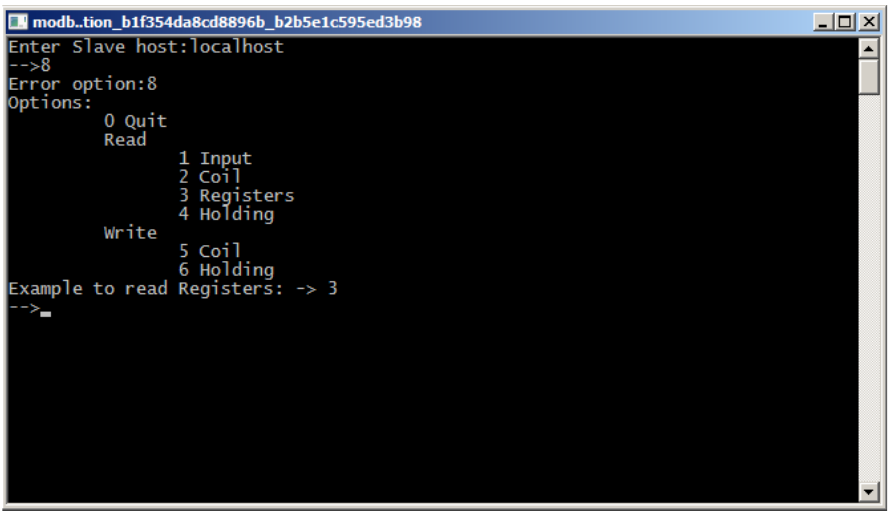
\includegraphics[width=\textwidth]{img/cliente_modbus.png}
\caption{\label{cliente_mod}Opciones funcionamiento de la aplicación de prueba que hace la función de cliente \emph{modbus}, abarcando todas las características del protocolo \emph{modbus}.}
\end{center}
\end{figure}

\subsection{Aprendizaje de las herramientas de la empresa}

Llegado a cierto punto, la empresa decidió que sería conveniente ceder la biblioteca que se emplea para el protocolo interno de comunicación con la impresora, junto el código,
brindando la oportunidad de conocer el funcionamiento del protocolo interno que emplea la empresa, siendo de gran ayuda en el futuro para el desarrollo del proyecto. Este código también dispone de su propia documentación donde explica el funcionamiento del \emph{PLC}, ayudando a comprender cómo funciona la aplicación interna, junto con los campos y los requisitos que requiere para su correcto funcionamiento. Además la empresa realizó una exposición de los componentes más útiles de la biblioteca para el desarrollo del proyecto, ayudando a su comprensión.

\subsection{Inicio del desarrollo del proyecto}

En este punto de la estancia en la empresa ya es posible empezar con el verdadero desarrollo del proyecto, disponiendo de los requisitos del proyecto de forma muy breve, los cuales fueron:

\begin{itemize}
\item El uso del protocolo \emph{modbus}.
\item El uso de la biblioteca interna.
\item Visualización de los resultados.
\item Estado del \emph{PLC}.
\end{itemize}

Una vez ya se tienen los requisitos del proyecto, se pudo empezar con el diseño de la aplicación, separándose en cuatro partes diferentes:

\begin{itemize}
\item La interfaz visual.
\item El apartado de comunicación con el \emph{PLC}.
\item Almacenaje de la información \emph{modbus}.
\item El intérprete del protocolo de la empresa.
\end{itemize}

También se aportaron ideas de nuevas funcionalidades que podría implementar la aplicación sin suponer un tiempo extra en su desarrollo. Estas características nuevas son:

\begin{itemize}
\item Añadir la opción de conectar la aplicación a un \emph{PLC} real, realizando así la función de un supervisor intermediario que sea capaz de visualizar la información que se envía entre el maestro y el \emph{PLC}.
\item Tener un registro de eventos de las conexiones realizadas al programa.
\item Guardar los datos de la aplicación para poder ser cargados en la aplicación en un futuro.
\end{itemize}

Todas estas extensiones fueron propuestas en la revisión del diseño, siendo aceptadas por el supervisor, permitiendo así su desarrollo para la aplicación.

\subsection{Diseño de la interfaz visual}

Para el diseño de la visualización de la aplicación se plantea inicialmente hacer un uso mediante consola, rechazándose inmediatamente esta propuesta al ver que el desarrollo de una interfaz mediante consola incrementa en exceso el tiempo destinado al desarrollo de la interfaz. Además, al tratarse de una aplicación para \emph{Windows}, la consola no ofrece la misma potencia que en otros sistemas operativos, como tampoco permite una interacción inmediata. Por tanto se decidió hacer una aplicación con interfaz gráfica requiriendo una variedad de posibles diseños que puede abarcar la aplicación, como se puede ver en el capítulo 4.3.

\subsection{Desarrollo de la etapa de almacenamiento}

El desarrollo de la aplicación empezó en el apartado de almacenaje de la información, al tratarse del punto central del cual dependerán el resto de elementos, además de requerir un formato especial que se asemeje lo más posible al protocolo \emph{modbus}. Al hacer uso de la biblioteca \emph{NModBus} esta parte del desarrollo se simplificó muchísimo al ya estar implementada y solo tener que prepararla para su uso con el resto de componentes creando funciones de lectura y escritura que facilitaran el acceso a la biblioteca.

\subsection{Desarrollo de la comunicación modbus}

El siguiente elemento a desarrollar del esquema de diseño es la comunicación, al pensar que es el apartado más difícil al tener que comunicarse con programas externos, siendo este trabajo facilitado principalmente por la biblioteca \emph{NModBus4}. Una particularidad al emplear tanto el almacenamiento como la comunicación la biblioteca \emph{NModBus4} es que dicha biblioteca ya está preparada para estas características lo que ha facilitado en gran medida el trabajo.

En este apartado principalmente nos hemos tenido que encargar de dar la opción de permitir que el programa abra la comunicación con el resto de programas o rechazarla, aparte de generar un evento que sea capaz de avisar en cada conexión recibida para el registro de eventos u otras necesidades.

\subsection{Desarrollo a partir de la biblioteca de la empresa}

A continuación se desarrolló el apartado que tiene que ver con el protocolo de la empresa, ya que una vez recibido y adaptado al caso de la aplicación que se desarrolla, realizando una implementación sencilla, surgió la problemática de ser necesario un fichero de configuración de la empresa requerido por la biblioteca.

La empresa cede un fichero de ejemplo \emph{json} con el cual se puede continuar trabajando. En el fichero \emph{json} se encuentran las posiciones \emph{modbus} de acceso importantes para poder visualizar las posiciones que accede y modifica el programa. También dicho fichero contiene los permisos de cada posición (lectura, escritura y lectura/escritura), así como información que se pueda tener en cuenta a la hora de continuar desarrollando esta parte o tener en cuenta posibles errores que puedan aparecer. Este fichero es importante para no romper el sistema del \emph{PLC} que está en la posible impresora física a la que la aplicación se puede conectar, ya que el \emph{PLC} de la impresora tiene la configuración de ese fichero. Se desarrollan a partir de la biblioteca dos partes distintas, una que simula el \emph{PLC} y la otra que permite conectarse conecta al \emph{PLC} físico que se encuentra en una impresora para gestionar correctamente las conexiones. De esta forma, el programa que se comunique con la aplicación desarrollada deberá emplear el mismo protocolo, dependiente del fichero de configuración.

\subsection{Desarrollo de la interfaz de la aplicación}

Se empieza con la herramienta gráfica que dispone \emph{Visual Studio} para el desarrollo. Esto facilita mucho el trabajo para plasmar la idea gráfica que se tiene inicialmente, como vemos en el capítulo 4.3. La aplicaciones tienen botones de función, campos para rellenar y la lista de las posiciones a las que ha de acceder el programa, el cual parte del fichero \emph{json}, un fichero donde se encuentra la configuración del protocolo de la empresa. Se tuvo un problema cuando se quería interactuar con la lista, ya que no se disponía del suficiente conocimiento como para que al pulsar encima de una fila de la lista se pudiera modificar un elemento de ésta.

Al explicar este problema a mi tutor, me explicó que para eso debería utilizar una biblioteca llamada \emph{MVVM Light Toolkit}, ya que es como se trabaja en la empresa. Por tanto se tuvo que empezar de nuevo la parte de la interfaz, empleando esta vez la biblioteca \emph{MVVM Light Toolkit}, la cual no era muy distinto de la forma sin la biblioteca, simplemente añade facilidades que ayudan a ahorrar tiempo.

El uso de esta biblioteca no ayudó a resolver el problema en la forma en la que se quería hacer. Lo que sí dio fue una solución alternativa y resolutiva para resolverlo por otra vía a la diseñada inicialmente que es la de crear una ventana emergente. Cada vez que se pulsa la fila del elemento el cual se quiere modificar, muestra todos los campos de dicho elemento y permite, si se da el caso, poder modificar los valores de dicho elemento. %¿cual?

\subsection{Unión de todas las piezas, desarrollo del núcleo}

Para unir todas las partes de la aplicación se ha empleado una clase que comunicará el almacenamiento de la aplicación con las distintas partes. Inicialmente se han encontrado muchos errores con el entorno visual de la aplicación, como:

\begin{itemize}
\item Botones que no funcionan correctamente.
\item Cambios de estado incorrectos.
\item La aplicación se cerraba al saltar excepciones no contempladas.
\item Modificaciones de valores en lugares no correspondientes.
\item Aparece más de una ventana emergente.
\item Fallos en el apartado de conectividad sin ni siquiera utilizarlo.
\end{itemize}

Todos y cada uno de estos fallos que no permitían el correcto funcionamiento básico de la aplicación fueron resueltos, consiguiendo que la aplicación resultara estable sin realizar ningún tipo de comunicación por red.

\subsection{Detección de errores de conectividad}

\subsubsection{Errores de la aplicación como esclavo}

Para poder comprobar posibles errores de conectividad, se pasó a probar la aplicación con un maestro sencillo que emplea el protocolo \emph{modbus}. El maestro \emph{modbus} a utilizar es la aplicación de prueba desarrollada anteriormente. Se comprobó tanto con opciones de lectura como de escritura desde el maestro.

Cuando se hicieron este tipo de pruebas, se vio la necesidad de crear eventos en la parte de comunicación para que activamente actualice automáticamente la información cada vez que recibe una solicitud de escritura, para que de esta forma aparezca la información del programa en la interfaz del usuario instantáneamente conforme se recibe, cosa que no se tuvo en cuenta en su momento.

También se pensó que este avance es de gran ayuda cuando queramos que el programa haga de intermediario entre \emph{PrintNuc} y el \emph{PLC}, añadiendo la funcionalidad de enviar la información al esclavo, cuando se pide una modificación, puesto que antes la aplicación no tenía esta opción de desarrollo.

\subsubsection{Errores de la aplicación como maestro}

En este caso la aplicación se ha de conectar a un esclavo. Para ello empleamos la aplicación \emph{ModbusPLCSimulator} que es de fácil manejo se dispone de conocimiento del protocolo \emph{modbus}. Se puede encontrar más información de la aplicación en el capítulo 2.11.

Cuando activamos esta opción, la aplicación se pone en marcha automáticamente a escuchar en un puerto el esclavo \emph{modbus}, mostrando los valores que tiene en ese instante el esclavo, actualizándolos cada vez que se modifica un valor.

De esta forma empezamos a comprobar que las limitaciones de escritura impuestas que no están permitidas se cumplen, comprobando que cada escritura y lectura las realiza correctamente, exceptuando por un error que ocurre cuando intenta modificar un valor de escritura que es de lectura.

El error detectado es debido a que en la biblioteca \emph{NMobdus4} la forma de almacenar no empieza en cero, como hace el estándar del protocolo \emph{modbus}, con lo cual, para solucionar el error se incrementa en uno, cada vez que se accede al dato, para que de esta forma la posición coincida con a la posición a la que se quiere acceder. Por eso se generaba el error de intentar modificar un valor que no se corresponde con los permisos de lectura/escritura estipulados.

\subsubsection{Errores de la aplicación como esclavo y maestro}

En este caso se comprueba el uso de estos tres programas, la propia aplicación, el maestro \emph{modbus} y el \emph{ModbusPLCSimulator}. Después de realizar un conjunto de pruebas, el uso es aceptable y sin errores. Esto hace tomar la decisión de mostrar la aplicación al supervisor para comprobar que el funcionamiento es igual de correcto que con la aplicación propia.

\section{Verificación y validación}

\subsection{Puesta en marcha con caso real}

En la puesta en marcha de la aplicación junto con la aplicación de la empresa, observamos que la aplicación no se conecta, cosa que sorprende, ya que la otra aplicación de prueba sí que funciona. La empresa cede su aplicación, que denominaremos \emph{PrintNuc}, para hacer pruebas sin depender del supervisor, para que pueda comprobar el por qué del funcionamiento incorrecto.

\subsection{Solución de la problemática de conexión}

Para descubrir que ha podido fallar, ha sido necesario emplear la aplicación \emph{Wireshark}, que se puede ver en el capítulo 2.12, para analizar las conexiones que realizan entre los programas y poder tener una idea de cuál es el fallo. Se descubre que el fallo es de interpretación del nombre de la máquina por una mala configuración, no abre los puertos en todas las direcciones que tiene la máquina en ese instante. La solución es cambiar la configuración para que abra los puertos en todo el rango de direcciones en las que se encuentra el ordenador en el que se ejecuta la aplicación.

\subsection{Comprobación del correcto funcionamiento}

\subsubsection{Conexión de la aplicación como esclavo}
En este punto se consigue conectar \emph{PrintNuc} correctamente a la aplicación, con una gran cantidad de peticiones por segundo que apenas se pueden ver debido a la gran velocidad que se generan y se reciben, sin generar ningún error a simple vista y comprobando que los valores que solicita leer y escribir el \emph{PrintNuc} en cada identificador corresponde correctamente con los que se muestran en la aplicación.

\subsubsection{Conexión de la aplicación como esclavo y maestro}
Además de conectar la aplicación a \emph{PrintNuc}, conectamos nuestra aplicación al \emph{ModbusPLCSimulator} para comprobar que los valores son los mismos que envía \emph{PrintNuc} y recibe \emph{ModbusPLCSimulator} a través de nuestra aplicación como intermediario. Aquí se ve que algo raro está ocurriendo, la aplicación que se está desarrollando no funciona con suficiente fluidez, funcionando a tirones, con problemas en la comunicación, ya que no llega toda la información porque los tirones generan que se pierdan paquetes de conexión con \emph{PrintNuc}, además de que en la aplicación \emph{PrintNuc} se muestra que la conexión está desconectada.

\subsubsection{Solución de errores de rendimiento}


Empezamos a investigar a qué se debe la pérdida de paquetes. Se encontró que el problema que generaba el fallo es por un problema de diseño de la aplicación, ya que por cada petición que recibe, manda una gran cantidad de peticiones al esclavo para leer la información, una por cada elemento que muestra por pantalla, generando un importante cuello de botella en la red.

Para solucionar este problema, se cambia la forma en la que se refresca la información en la pantalla, para que así no tenga que hacer una petición para actualizar la información con cada elemento que se cambie el valor. A partir de este instante, la información que se muestra por la pantalla, no solicita la actualización de todos los datos al instante.

\subsection{Comprobación de fluidez y comprobación de correcto funcionamiento}

En esta nueva prueba se comprueba que el funcionamiento de la aplicación mejora en todos los aspectos de fluidez en los distintos modos de funcionamiento que tiene. Se vuelven a comprobar todos los parámetros de funcionamiento de las tres aplicaciones, con las distintas variables, comprobando que todo funciona según los requisitos.

Cuando se comparan los datos que envía \emph{PrintNuc} y son recibidos por \emph{ModbusPLCSimulator} se observa que algunos datos son correctos, en cambio otros se encuentran como desplazados en potencias base 10 a la derecha o a la izquierda.

\subsection{Solución de error de datos}

Se empieza a analizar el problema comprobando qué cálculo hace la aplicación para hacer estos desplazamientos. Con la lectura del código de  la biblioteca de la empresa, se descubre que hay un apartado que se encarga de esa función.

Como anteriormente se ha hecho, se vuelve a poner en marcha \emph{PrintNuc} y \emph{ModbusPLCSimulator}, para comprobar cuál es la diferencia entre la información inicial emitida y la final recibida, observando que la tarea del desplazamiento en base 10 se hace dos veces, una vez cuando la aplicación recibe el valor, almacenándose en nuestro programa desplazado y este mismo valor nuestra aplicación lo vuelve a desplazar para enviar al esclavo de nuevo.

Para solventar este error, se realiza la conversión de nuevo en formato que la biblioteca de la empresa pueda enviar correctamente la información al esclavo. De esta forma conseguimos corregir el error que provocaba la aplicación, enviando, ahora sí, correctamente los datos del programa a \emph{ModbusPLCSimulator}.

\subsection{Comprobación final}

Se vuelve a hacer una comprobación exhaustiva de la aplicación, añadiendo nuevas pruebas de estabilidad. Estas pruebas de estabilidad consisten en hacer frente a una detención inesperada del maestro y/o el esclavo, cerrando forzosamente en el sistema las aplicaciones \emph{PrintNuc} y/o \emph{ModbusPLCSimulator} con las que mantiene una conexión en red.

Esta última comprobación ha generando en ocasiones que la aplicación fallara y en otras no, descubriendo que se trata de un problema de salto de excepción al interrumpir el hilo en el que se encuentra ese momento la conexión. La solución a este problema ha sido que cada vez que se detectaba que la conexión se interrumpía bruscamente, finalizar el hilo correctamente para evitar que se siga ejecutándose él mismo y también se ha capturado la excepción para que no afecte al resto del sistema, de esta forma pueda continuar el correcto funcionamiento del programa.

\chapter{Funcionamiento de la aplicación}

\section{Requisitos}
Para su funcionamiento, la aplicación requiere de un fichero <<\emph{*.JSON}>> específico, puesto que este fichero contiene los parámetros de funcionamiento de la aplicación simulada, los mismos que va a emplear el maestro. Este fichero es escogido por defecto en la carpeta donde se encuentra la aplicación y en caso de no encontrarse, se solicita el fichero al usuario. Si no se selecciona ningún fichero, la aplicación se cierra. 

\section{Interfaz de la aplicación}
Como se puede observar en la Figura \ref{func_apli}, la aplicación dispone de una interfaz dinámica en la que se observan todos los cambios instantáneamente.

\begin{figure}
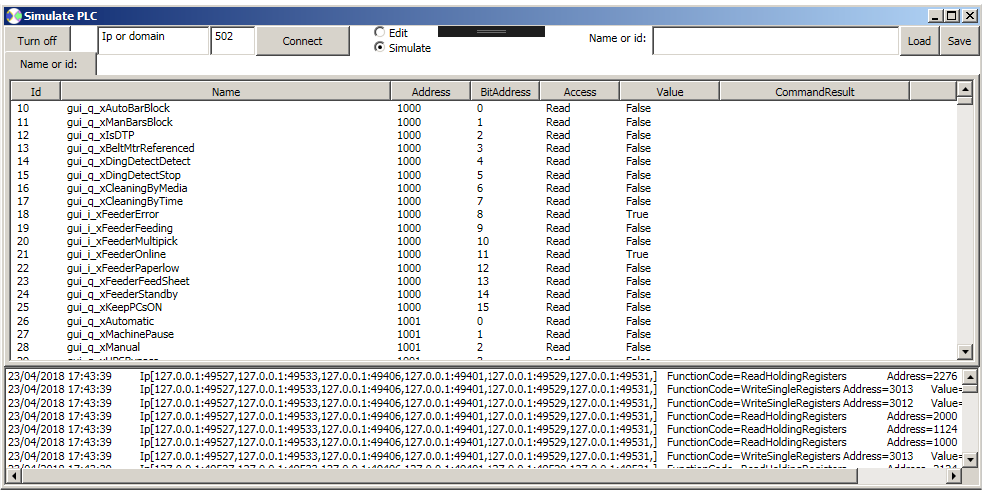
\includegraphics[width=\textwidth]{img/disenyo_ui2.png}
\caption{\label{func_apli}Aplicación en funcionamiento.}
\end{figure}

Con este aspecto se ha intentado que la aplicación sea lo más autodescriptiva posible, para su mayor facilidad de uso. Se puede ver que  dispone de tres zonas claramente diferentes:

\begin{itemize}
\item La \textbf{zona superior} donde se consideran los elementos de control de la aplicación, en la cual se permite cambiar el funcionamiento de la misma.
\item La \textbf{zona central} donde se encuentran los datos del \emph{PLC} simulado o real y se permite editar dichos datos.
\item La \textbf{zona inferior} la cual es un registro de las conexiones que han realizado otros maestros a nuestra aplicación mediante el protocolo \textbf{modbus}, que también se almacenan en un fichero.
\end{itemize}

A continuación se procederá a explicar qué función realiza cada uno de los botones de la zona superior de la aplicación, las cuales son:

\textbf{Identificar en las imágenes y en la lista}

\begin{enumerate}[a)]
\item Poner en marcha o en espera el servidor \emph{modbus} de la aplicación.
\item Conectar a un servidor \textbf{modbus} para retransmitir todas las comunicaciones recibidas desde el cliente.
\item Activar o desactivar el  modo de edición, visualización o simulación de la aplicación.
\item Filtrar rápidamente por nombre o identificador.
\item Almacenar o cargar el estado de las variables de cada campo.
\end{enumerate}

Estas explicaciones también se encuentran en la Figura \ref{izquierda} para la zona izquierda de control de la aplicación y en la Figura \ref{derecha} para la parte derecha de la aplicación. 

\begin{figure}
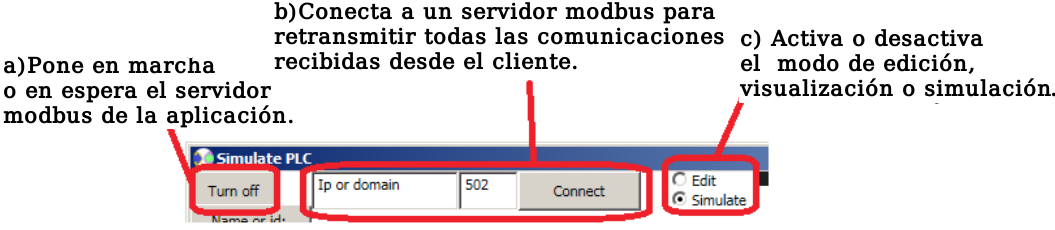
\includegraphics[width=\textwidth]{img/exp1.png}
\caption{\label{izquierda}Funcionamiento de cada botón de la zona superior izquierda.}
\end{figure}


\begin{figure}
\begin{center}
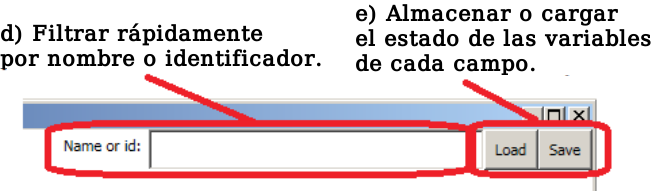
\includegraphics[width=0.69\textwidth]{img/exp2.png}
\caption{\label{derecha}Funcionamiento de cada botón de la zona superior derecha.}
\end{center}
\end{figure}

Además cabe indicar que al pulsar cualquier dato en el apartado del centro, aparece una ventana que da la opción para la edición del valor si es posible en ese preciso instante. La ventana que se muestra es la de la Figura \ref{datos}, y como podemos observar se da la opción de modificar el dato o de cancelar dicha modificación. Dicho valor cuando se trata de una variable booleana solo acepta <<False>> , <<false>> o <<0>> como valor negativo, considerando positivo cualquier otro valor.

\begin{figure}
\begin{center}
\includegraphics[]{img/disenyo_emergente.png}
\caption{\label{datos}Esta ventana permite modificar los datos y ver las características del elemento.}
\end{center}
\end{figure}

\section{Otras características a tener en cuenta}

Hay que tener en cuenta que cada vez que se pone en ejecución el programa, la aplicación genera un fichero en la carpeta donde se encuentra el ejecutable. En este fichero se encuentra un registro de las conexiones que han realizado otros maestros a nuestra aplicación mediante el protocolo \emph{modbus}.



\chapter{Conclusiones}
%Se pueden presentar conclusiones en varios aspectos: 
%en el ámbito formativo (sobre lo que has aprendido),
%en el ámbito profesional (sobre la experiencia en la empresa)
%y en el ámbito personal (sobre tu experiencia personal).
%En las conclusiones, además de las consideraciones personales, académicas o profesionales que el alumno quiera comentar, 
%se pueden incluir posibles extensiones del proyecto, así como la viabilidad comercial o empresarial cuando proceda.

Durante el desarrollo de la aplicación, se han adquirido nuevas competencias que se desconocían, como la resolución rápida de conflictos, la capacidad de documentar aplicaciones y las sinergias de trabajar con otros departamentos.

Además la aplicación ha conseguido evolucionar más sin la necesidad de emplear mucho tiempo en su desarrollo, añadiendo funcionalidades como puede ser realizar un volcado de datos a un fichero, tener un control de registros de eventos de las solicitudes recibidas y almacenarlas en un fichero intermediario entre la aplicación y el \emph{PLC}. No solo se han cumplido los objetivos básicos inicialmente establecidos, sino que además se han incluido otros que pueden ser de gran ayuda.

Sin embargo, en una futura revisión, se deberían corregir algunas carencias del sistema:
\begin{itemize}
\item Simulación del \emph{PLC} más real.
\item Añadir control de versión del \emph{PLC}.
\item Permitir almacenar los datos en la ubicación que el usuario desee.
\item Permitir leer los datos en la ubicación que el usuario desee.
\item Permitir cambiar el puerto de escucha por defecto.
\item Permitir almacenar una copia del registro de eventos.
\item Autoaprendizaje mediante inteligencia artificial para simular con la mayor precisión posible.
\end{itemize}


% ------------------- Bibliografia ---------------------
\addcontentsline{toc}{chapter}{Bibliografía}
%\bibliographystyle{plane}
%\bibliography{MemoriaTecnicaBibliografia.bib}

\begin{thebibliography}{X}
\bibitem{plc_wiki}
 \textsc{Comunidad wikipedia},
 \textit{Controlador lógico programable},
 \url{https://es.wikipedia.org/wiki/Controlador_l%C3%B3gico_programable},
  26 de junio de 2018.
\bibitem{plc}
 \textsc{Machine-Information-Systems.com},
 \textit{What IS a PLC?},
 \url{http://www.machine-information-systems.com/PLC.html},
  26 de junio de 2018.
\bibitem{scrum}
 \textsc{Ikujiro Nonaka} y \textsc{Hirotaka Takeuchi},
 \textit{The New New Product Development Game},
 1986
\bibitem{jira}
 \textsc{Atlasian},
 \textit{página web},
 \url{https://es.atlassian.com/software/jira},
  26 de junio de 2018.
\bibitem{json}
 \textsc{Douglas Crockford},
 \textit{Internet JSON},
 \url{https://tools.ietf.org/html/rfc7493},
  26 de junio de 2018.
\bibitem{visual_studio}
 \textsc{Microsoft},
 \textit{página web},
 \url{https://visualstudio.microsoft.com/es/},
  31 de marzo de 2018.
\bibitem{c_sharp}
 \textsc{Microsoft},
 \textit{página web},
 \url{https://docs.microsoft.com/dotnet/csharp/language-reference/},
  26 de junio de 2018.
\bibitem{wpf}
 \textsc{Microsoft},
 \textit{XAML Overview (WPF)},
 \url{http://msdn.microsoft.com/en-us/library/ms752059.aspx},
  26 de junio de 2018.
\bibitem{mvvm}
 \textsc{Josh Smith},
 \textit{WPF Apps with the Model-View-ViewModel Design Pattern},
 \url{https://docs.microsoft.com/dotnet/csharp/language-reference/},
  26 de junio de 2018.
\bibitem{mvvmlight}
 \textsc{MVVM Light Toolkit group},
 \textit{página web},
 \url{http://www.mvvmlight.net/doc},
  26 de junio de 2018.
\bibitem{git}
 \textsc{Scott Chacon} y \textsc{Ben Straub},
 \textit{Pro git},
 \url{https://git-scm.com/book/en/v2}
\bibitem{modbus}
 \textsc{Modbus Organization},
 \textit{MODBUS Protocol Specification},
 \url{http://modbus.org/docs/Modbus_Application_Protocol_V1_1b3.pdf},
  26 de junio de 2018.
\bibitem{modbustcp}
 \textsc{Modbus Organization},
 \textit{MODBUS TCP/IP},
 \url{http://modbus.org/docs/Modbus_Messaging_Implementation_Guide_V1_0b.pdf},
  26 de junio de 2018.
\bibitem{nmodbusapi}
 \textsc{Lin, Renee},
 \textit{NModbus API Manual, versión 1.2}
 \url{http://ftp.icpdas.com/pub/cd/8000cd/napdos/modbus/nmodbus/nmodbus_api_manual_v1.2_en.pdf},
  26 de junio de 2018.
\bibitem{plcsimulator}
 \textsc{zaphodikus},
 \textit{About the Author}
 \url{http://www.plcsimulator.org/Home/about},
  26 de junio de 2018.
\bibitem{wireshark}
 \textsc{The Wireshark team}
 \textit{Página web de Wireshark}
 \url{https://www.wireshark.org/},
  26 de junio de 2018.
\bibitem{pc}
 \textsc{Ordenador HP Pavilion Power 570-P044NS}
 \url{https://www.pccomponentes.com/hp-pavilion-power-570-p044ns-amd-a10-9700-16gb-1tb-gtx-1050},
  26 de junio de 2018.
\bibitem{monitor}
 \textsc{Monitor Samsung S24D330}
 \url{https://www.coolmod.com/samsung-s24d330-24-led-monitor-precio},
  26 de junio de 2018.
\bibitem{raton}
 \textsc{Ratón L-Link LL-2080-R}
 \url{https://www.coolmod.com/l-link-ll-2080-r-negro-rojo-ratan-precio},
  26 de junio de 2018.
\bibitem{teclado}
 \textsc{Teclado Kloner KTU20}
 \url{https://www.coolmod.com/kloner-ktu20-usb-negro-teclado-precio},
  26 de junio de 2018.
\bibitem{internet}
 \textsc{Netllar Internet 30}
 \url{https://www.netllar.es/internet-fibra-optica/}
\bibitem{salario},
  26 de junio de 2018.
 \textsc{Tusalario.es},
 \textit{página web},
 \url{http://tusalario.es},
  26 de junio de 2018.
\end{thebibliography}


% ------------------- Anexos ---------------------

\appendix
%\renewcommand\appendixname{Anexo}

% ---- Primer Anexo ----
%\chapter{Estudio detallado de...}

%\section{Definición}

%\section{Aplicaciones}

% ---- Segundo Anexo ----
%\chapter{Tablas de ...}

\end{document}
